%%
%% Template chap2.tex
%%

\chapter{Experiment 1: Learning with Random Sampling}
\label{cha:expt1}

Before we can get to the main investigation of Thompson sampling in Chapter \ref{cha:expt2},
we need to first prepare the datasets and experiment with random sampling. The goal of
this chapter is to do feature selection and compare the performance of various standard
classifiers. This, in turn, will help us design the protocol
of the active learning experiment.

\section{Preparation of Data}

The VST ATLAS dataset has been specifically prepared for us by Christian Wolf so there
is no need to do any cleaning or feature selection.
The SDSS dataset, on the other hand, was extracted from the Sloan SkyServer. Appendix
\ref{cha:datasets} contains the SQL queries and instructions on how to replicate
the data. In particular, we extract two sets of data.
For the labelled objects, we only include those that have a clean
spectrum and hence a reliable spectroscopic label. We do not impose any limit on how faint
an object can be, but we do exclude those with a photometric error greater than 3 mag (i.e.
3 orders of magnitudes in brightness). This is deliberate since this allows us to 
investigate how well our classifiers can deal with noisy data.
Given the constraints, the resulting labelled set contains
2.8 million objects. Finally, the second set of SDSS data contains photometric measurements
of all 800 million objects in the database. No constraints were applied to this set.

Originally, each object contains 5 PSF and 5 Petrosian magnitudes.
However as we discussed
in \ref{sub:colours}, these magnitudes are dependent on distance. To remove this
dependency,  we take 
the differences and obtain the colours. By convention, we calculate the $u-g$, $u-r$, $r-i$,
and $i-z$ colours. In addition, we keep one apparent magnitude in the set of features.
The magnitude in the r-band is chosen since it lets the the greatest fraction of light through
the filter. This, hopefully, would give us a high signal-to-noise ratio.
Although it has been not been rigorously verified, this combination of four colours and
one magnitude has been found to produce good results by astronomers in the past [Wolf, pers. comm.].
In the end, we end up with 11 features:
\begin{itemize}
	\item Four PSF colours ($u-g$, $u-r$, $r-i$, $i-z$) and the r-band PSF magnitude.
	\item Four Petrosian colours ($u-g$, $u-r$, $r-i$, $i-z$) and the r-band Petrosian magnitude.
	\item The r-band Petrosian radius.
\end{itemize}
For a quick visualisation of these features, we make a scatter
plot in Figure \ref{fig:sdss_pca_all}
the first two principal components. Although we can clearly see clusters of stars, quasars, 
and galaxies, there is also enough  overlapping between classes, especially between
stars and quasars, the make the problem interesting.

\begin{figure}[tbp]
	\centering
	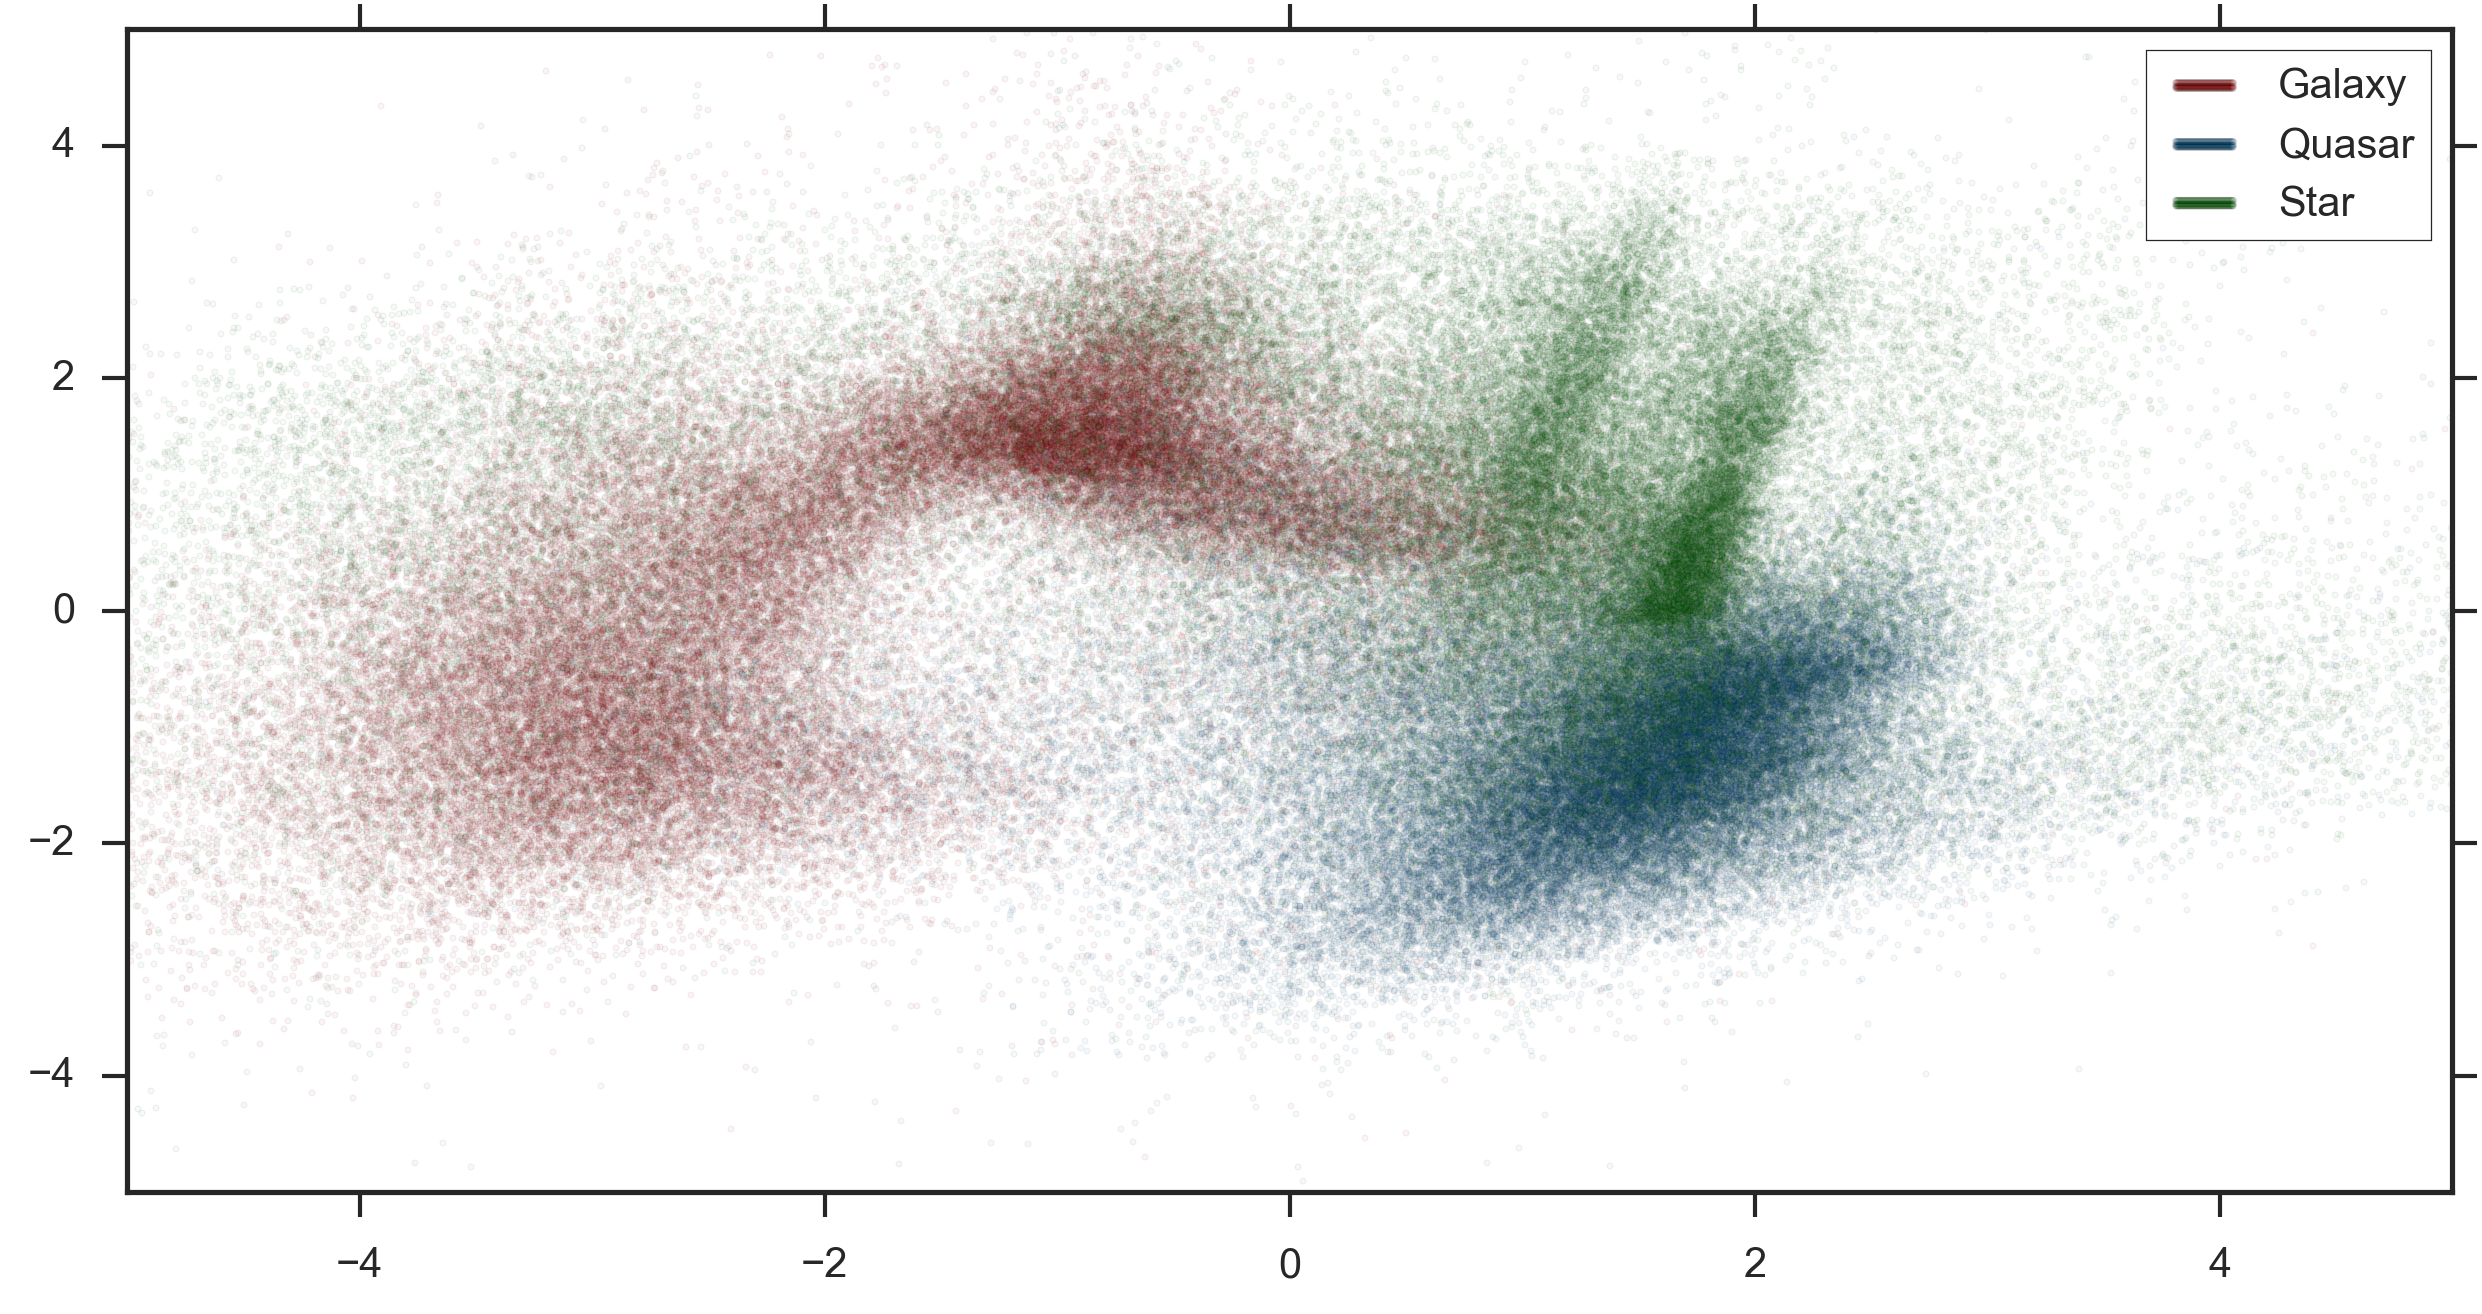
\includegraphics[width=\textwidth]{figures/4_expt1/sdss_pca_all}
	\caption[First two principcal components of the SDSS dataset]{We use principal
		component analysis (PCA) to reduce the 11 features of the SDSS dataset down
		to two dimensions. This allows us to do a quick visual scan and see how
		separable the three classes are.}
	\label{fig:sdss_pca_all}
\end{figure}


\section{Experimental Protocol}
\label{sec:protocol1}

This experiment consists of three parts. We first compare sets of reddening correction.
We then examine the performance of various classifiers with random sampling. Finally
we pick the best classifier and use it to predict the unknown proportion in the unlabelled
set.

\subsection{Reddening Correction}
In order to compare three sets of dust extinction, SDF98, SF11, and W14, we first
split the labelled pool into a balanced training set of size 600,000 and a balanced test
set of size 300,000. We then apply each a correction and train a random forest of 300 decision
trees. A random forest is chosen due to its speed. Finally the accuracy rate on the test set allows
us to decide on the best performing reddening correction set. This set will be applied
in all subsequent experiments.

\subsection{Copmaring Classifiers}
Next we would like to compare the performance of four classifiers: random forests, logistic
regression, linear SVMs, and SVMs with an RBF kernel. In the random forest,
we again build 300 trees and the
Gini impurity is used to measure the quality of a split. With the other classifiers,
there
are a few hyperparameters that require tuning before. To find the optimal values,
we conduct a search in the parameter space with logarithmic steps. For each combination,
we do a five-fold cross validation with a training and test size of 300 each. We then plot
the results on a heat map.

Out of the classifiers being tested, only random forests and SVMs with
an RBF kernel are capable of learning non-linear decision boundaries. Logistic regression
and linear SVMs, on the other hand, cannot. Thus for the latter two, we also do a degree
2 and degree 3 polynomial transformation of the features, which allows the linear classifiers
the learn more complicated hypotheses.

Once the hyperparameters are optimised, we compare the performance of the classifiers by looking
at their learning curves. The VST ATLAS data is fairly small, so we can use all of the examples.
Using all of the SDSS labelled examples would take too long on some classifiers like
logistic regression, we stop at 300,000 examples. To smooth out the curve, we do a
stratified shuffle split with 5 iterations, and then take average of the results.

Since we would like to use as much data as possible, no attempt is made to balance the classes.
Instead we give to the classifiers a weight vector that is proportional to the inverse
of the class frequencies. This means that rare objects like white dwarfs are given more
weight during training. In addition, we use the posterior balance accuracy rate to remove
any bias toward the dominant class.

Finally since we have 800 million unlabelled objects in the SDSS, let us pick the
best performing classifier and predict the class proportion on the unlabelled data.
In doing so, we using the numbers in the confusion matrix and try to correct for the
potential misclassification.

\section{Results and Discussion}
\label{sec:results1}

\subsection{Comparison of Reddening Correction Sets}
Figure \ref{fig:reddeningviolin} on page \pageref{fig:reddeningviolin} shows
the violin plot of the accuracy rate on the test
set when apply each of the three correction set. Appendix \ref{cha:supp} contains
more detailed maps on the improvement of the recall rate. Overall, the results are quite
uninteresting since no statistical differences can be found between the three sets. In fact,
even if we do not apply any correction, the accuracy rate still remains unchanged.

This is probably due to the fact that there are not too many objects in the Milky Way band,
the region in which there is the most dust extinction. Indeed, if we look back at the reddening map
in Figure \ref{fig:reddening}, the extinction amount does look fairly small and uniform
throughout the scanned region.
In any case, for good measure, we will correct all photometric measurement for dust
extinction using
the latest W14 set. Other projects like SkyMapper will survey regions closer to the Milky
Way band and thus future work using its data might be able to provide more conclusive
evidence of which of the three sets is the most effective.

\begin{figure}[tbp]
	\centering
	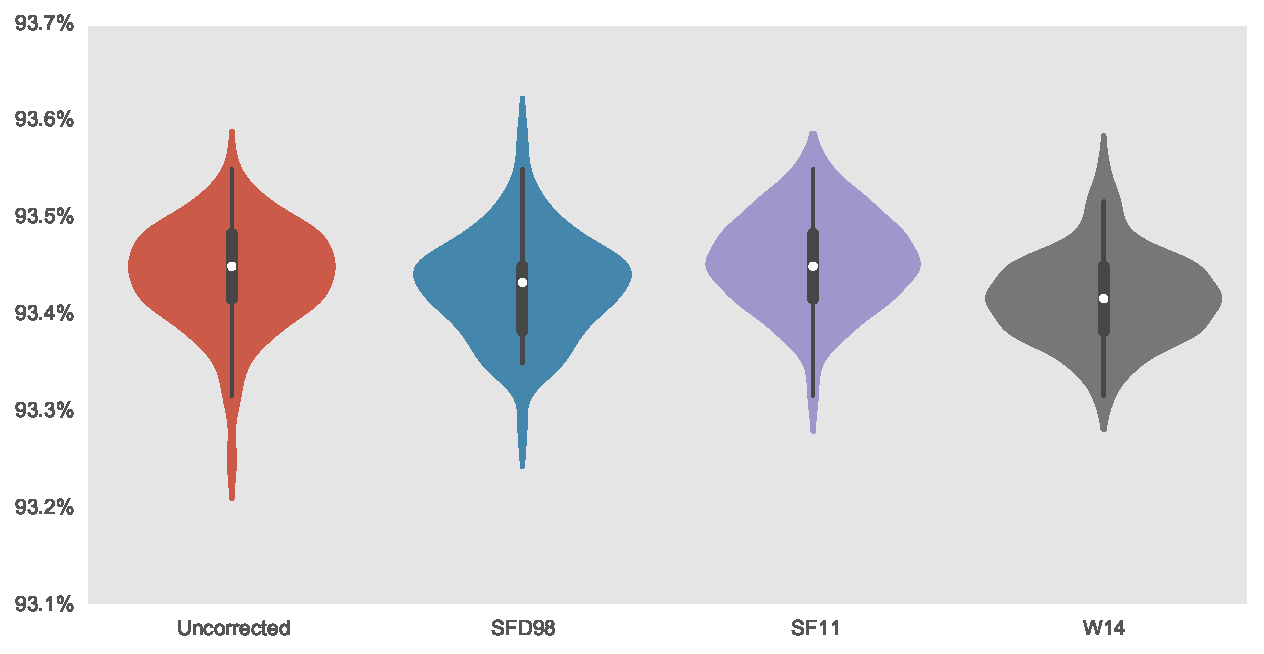
\includegraphics[width=\textwidth]{figures/4_expt1/violin_reddening_correction}
	\caption[Accuracy rates with four reddening correction sets]{Comparing the
		accuracy rates using 4 correction sets.}
	\label{fig:reddeningviolin}
\end{figure}

\subsection{Hyperparameters Optismations}
On the next three pages, we show the heat maps of the cross-validation accuracy rate
for many different combinations of hyperparameters. For readability, we provide detailed
reasoning under each figure of how we choose the optimal values of the parameters.
Below we provide a summary of our decisions:
\begin{itemize}
	\item \textbf{Logistic Regression}: We do first a degree 2 polynomial transformation of both
	the SDSS and the VST ATLAS features. For the classifier, we use the one-vs-rest
	strategy and an L1-norm for the penalisation, thus giving us sparse solutions. The inverse
	regularisation term $C$ is 1 in SDSS and 100 in VST ATLAS.
	\item \textbf{Linear SVM}: For the SDSS data, we also do a degree 2 polynomial transformation
	and our classifier uses the one-vs-rest strategy with the square hinge loss function
	and, an L1-norm, and $C=0.1$. For the VST ATLAS dataset, there is no need to do 
	any transformation and we use the Crammer-Singer approach.
	\item \textbf{SVM with RBF Kernel}: The optimal hyperameter values for the SDSS data are
	$\gamma = 0.01$ and $C = 1,000$. For the VST-ATLAS data, they are $\gamma = 0.001$ and
	$C = 1,000,000$.
\end{itemize}

\begin{figure}[p]
	\centering
	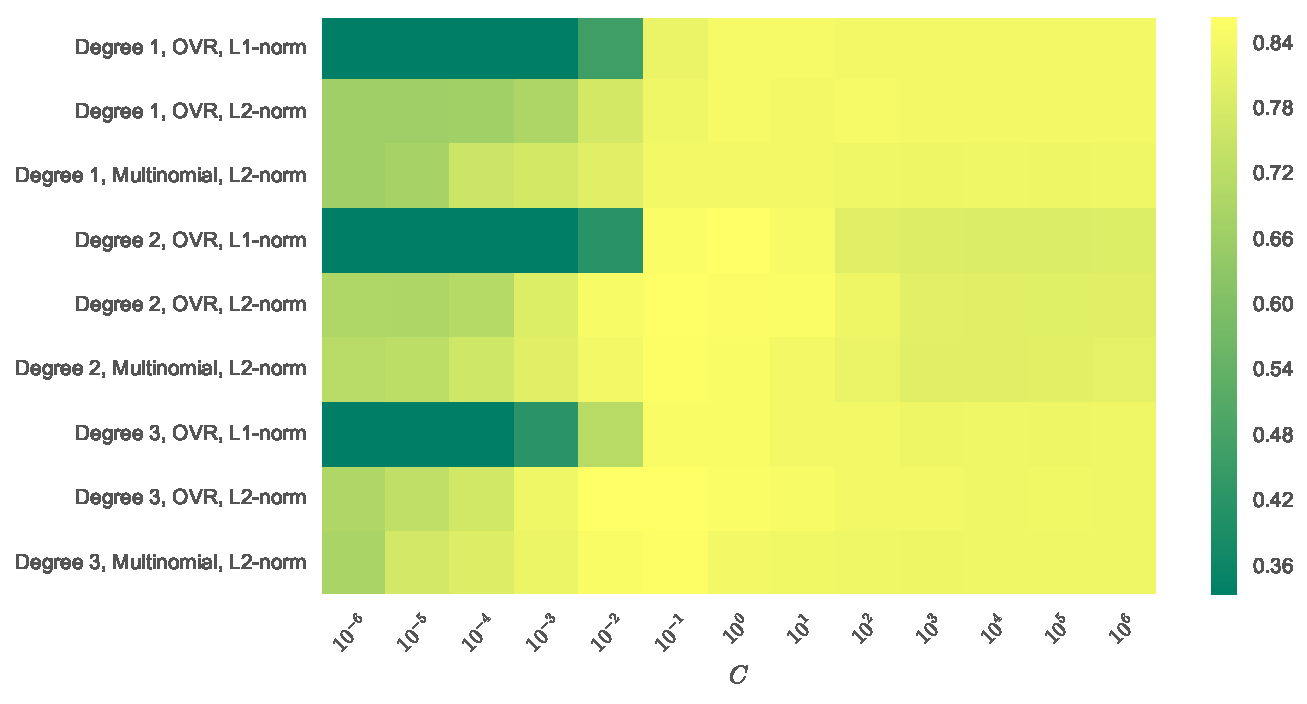
\includegraphics[width=\textwidth]{figures/4_expt1/sdss_grid_logistic}
	\caption[Heatmap of logistic regression's cross-valdiation accuracy in SDSS]{
		Heatmap of linear logistic regression's cross-valdiation accuracy in the SDSS dataset:
		The best-perfomring combination involves doing a degree 3 polynomial transformation
		of the features. In practice, this would make it too slow to run subsequent experiments.
		Thus we sacrifice a bit of accuracy and pick the optimal parameters that
		involve only a degree 2 polynomial transformation. In particular, we set the inverse regularisation
		term $C$ to be 1 and use the one-vs-rest strategy with L1-norm.}
	\label{fig:sdss_grid_logistic}
\end{figure}

\begin{figure}[p]
	\centering
	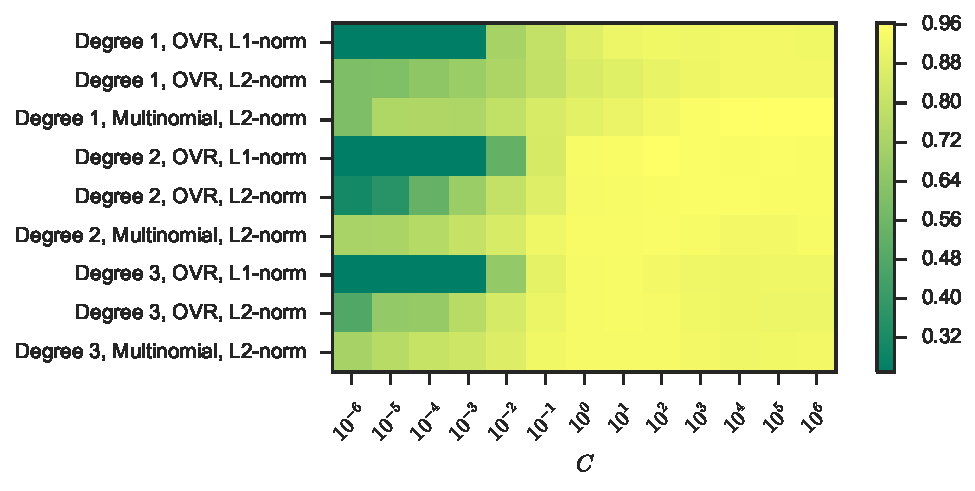
\includegraphics[width=\textwidth]{figures/4_expt1/vstatlas_grid_logistic}
	\caption[Heatmap of logistic regression's cross-valdiation accuracy in VST ATLAS]{
		Heatmap of logistic regression's cross-valdiation accuracy in the VST ATLAS dataset:
		The optimal combination invovles using multinomial logistic regression. This
		might seem like a good choice since we get true probability estimates. However
		it turns out that the Scikit-learn implementation of multinomial regression
		gives unstable probabilities. Thus we resort to the next best combination,
		where we use one-vs-rest, a degree 2 polynomial transformation of the features, and $C = 100$. }
	\label{fig:vstatlas_grid_logistic}
\end{figure}

\begin{figure}[p]
	\centering
	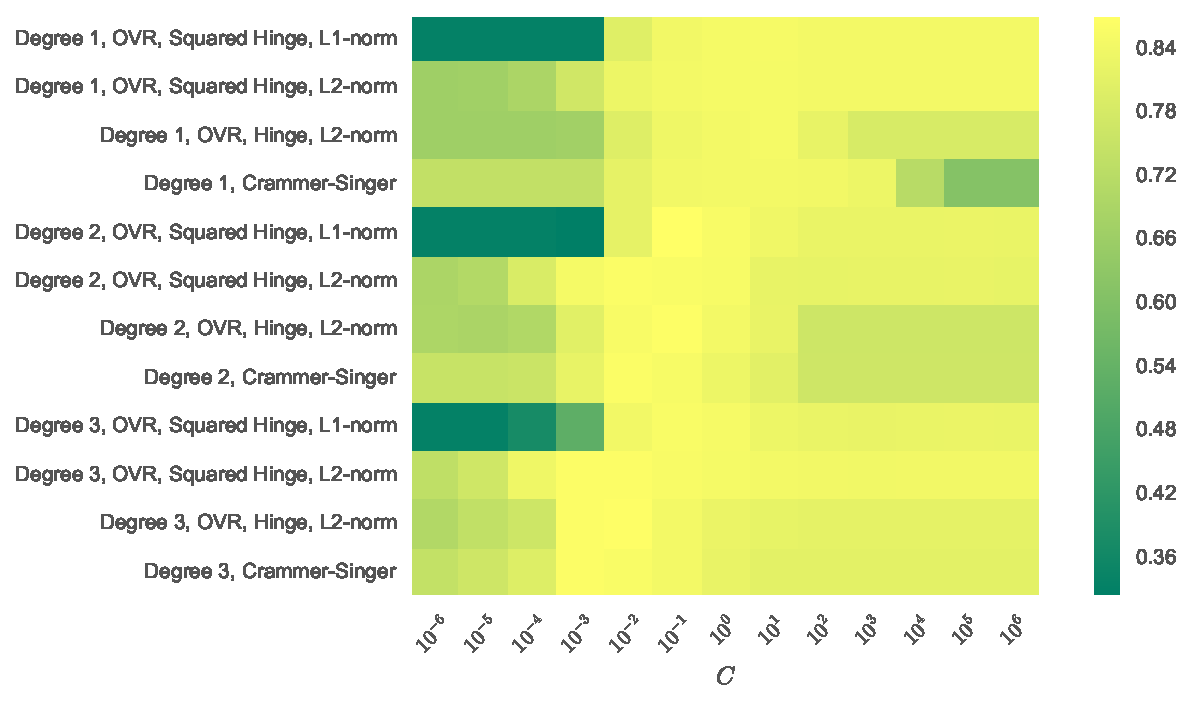
\includegraphics[width=\textwidth]{figures/4_expt1/sdss_grid_poly}
	\caption[Heatmap of linear SVM's cross-valdiation accuracy in SDSS]{
		Heatmap of linear SVM's cross-valdiation accuracy in the SDSS dataset:
		Like Figure \ref{fig:sdss_grid_logistic}, the optimal
		combination involves a degree 3 polynomial transformation of the features.
		Due to constraints on
		processing power, we will instead pick the next best alternative, which involves
		a degree 2 transformation, the one-vs-rest strategy, the square hinge loss function,
		and the L1-norm for the penalisation}
	\label{fig:sdss_grid_poly}
\end{figure}

\begin{figure}[p]
	\centering
	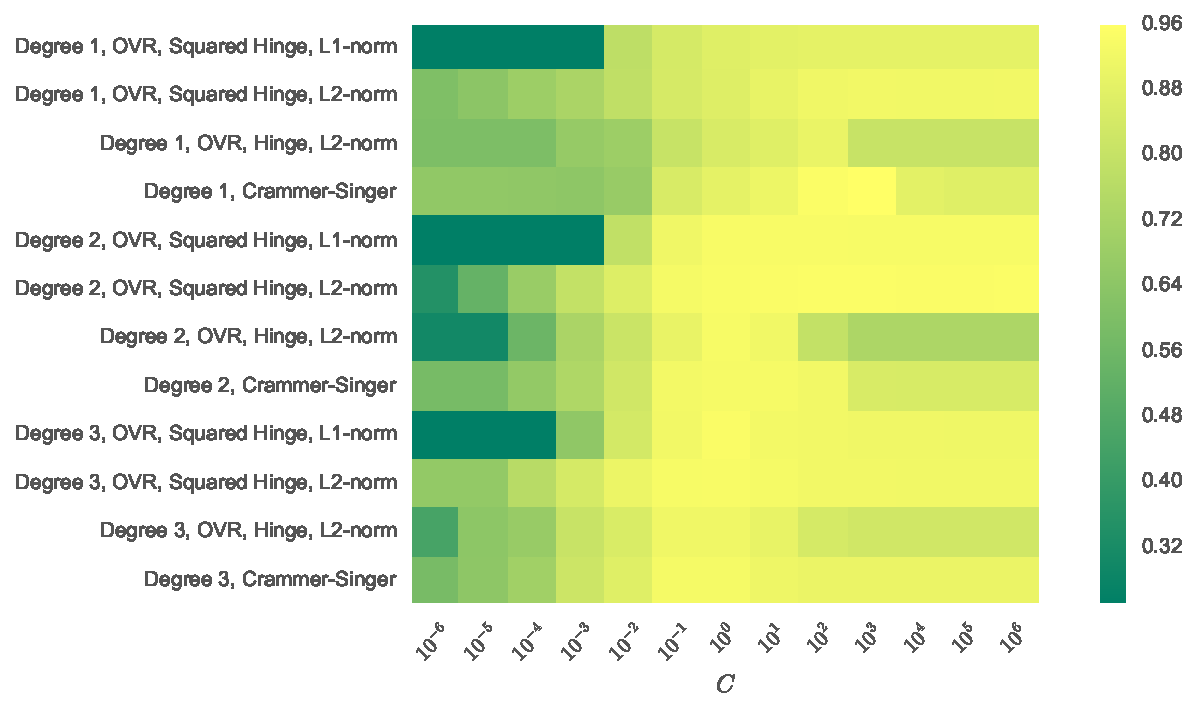
\includegraphics[width=\textwidth]{figures/4_expt1/vstatlas_grid_poly}
	\caption[Heatmap of linear SVM's cross-valdiation accuracy in VST ATLAS]{
		Heatmap of linear SVM's cross-valdiation accuracy in the VST ATLAS dataset:
		Interestingly, the optimal combination does not require any polynomial
		transformation of the features, and instead of the usual one-vs-rest strategy,
		we the Crammer-Singer method
		with $C = 1000$ gives the best result. In theory, the Crammer-Singer approach
		can give us true probability estimates, however this has not been implemented
		in Scikit-learn.}
	\label{fig:vstatlas_grid_poly}
\end{figure}

\begin{figure}[p]
	\centering
	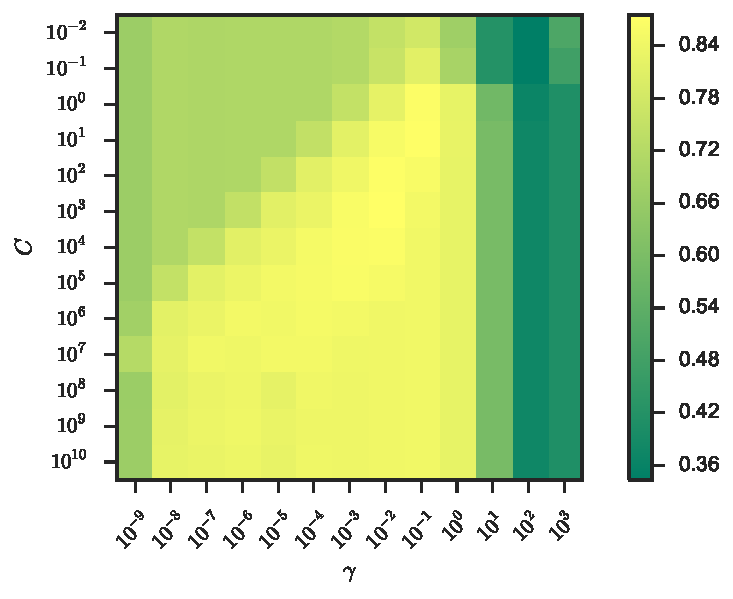
\includegraphics[width=0.7\textwidth]{figures/4_expt1/sdss_grid_rbf}
	\caption[Heatmap of RBF SVM's cross-valdiation accuracy in SDSS]{
		Heatmap of RBF SVM's cross-valdiation accuracy in the SDSS dataset:
		Here the optimal values for the hyperparameters are $\gamma=0.01$
		and $c = 1,000$, giving a accuracy of around $88\%$.}
	\label{fig:sdss_grid_rbf}
\end{figure}

\begin{figure}[p]
	\centering
	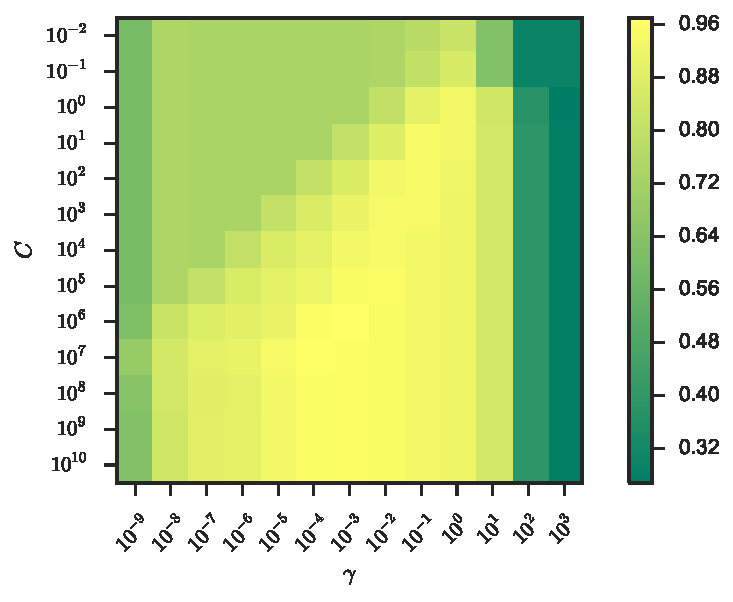
\includegraphics[width=0.7\textwidth]{figures/4_expt1/vstatlas_grid_rbf}
	\caption[Heatmap of RBF SVM's cross-valdiation accuracy in VST ATLAS]{
		Heatmap of RBF SVM's cross-valdiation accuracy in the VST ATLAS dataset:
		The optimal values are $\gamma=0.001$ and $C = 1,000,000$, giving us an accuracy
		of $97\%$. Observe that
		with a large value of $C$, we would need more support vectors during training
		and hence the the model will be somewhat slower at prediction.}
	\label{fig:vstatlas_grid_rbf}
\end{figure}


\subsection{Learning Curves with Random Sampling}
Now that we have tuned the hyperparameters, we are ready to compare the classifiers.
Figure \ref{fig:learning_curves} shows the average learning curves of the two datasets.
Overall the two best performers are random forests and SVMs with an RBF kernel. The VST ATLAS
data appears to be very clean, with highest achievable balanced accuracy rate of 99\%.
Logistic regression with a degree 2 polynomial transformation is the slowest algorithm,
surprising even slower than the RBF SVM.

\begin{figure}[tbp]
	\centering
	\begin{subfigure}{.5\textwidth}
		\centering
		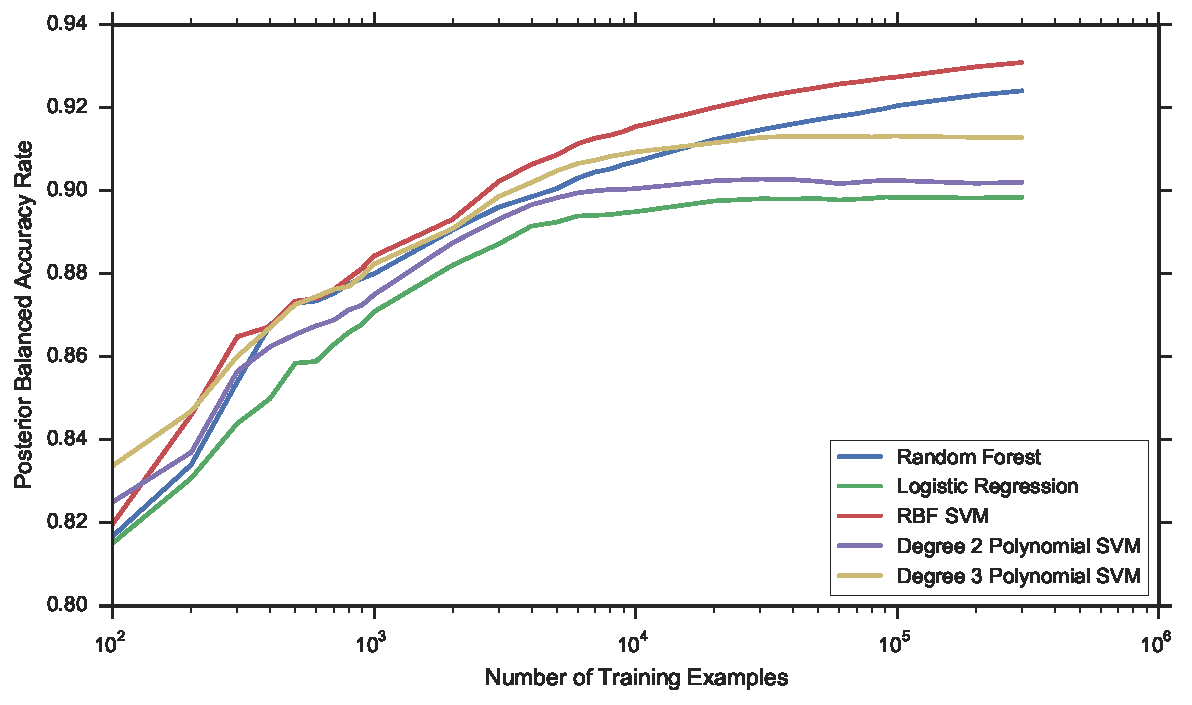
\includegraphics[width=0.99\textwidth]{figures/4_expt1/sdss_learning_curves}
		\caption{With SDSS data}
		\label{fig:sdss_learning_curves}
	\end{subfigure}%
	\begin{subfigure}{.5\textwidth}
		\centering
		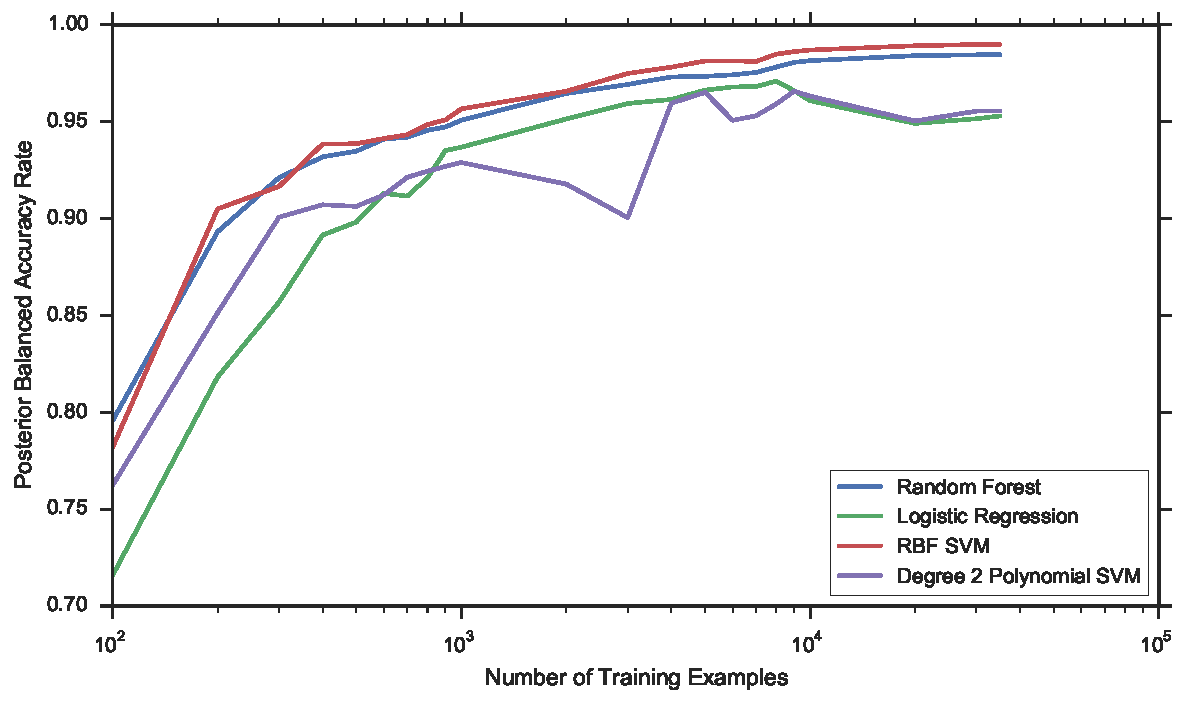
\includegraphics[width=0.99\linewidth]{figures/4_expt1/vstatlas_learning_curves}
		\caption{With VST ATLAS data}
		\label{fig:vstatlas_learning_curves}
	\end{subfigure}
	\caption[Learning curves with random sampling]{
		These are the average learning curves (of 5 trials) with random sampling.
		Note that we use a log scale for the y-axis since generally, it gets exponentially
		more difficult to improve the accuracy rate as we the accuracy approaches 1.}
	\label{fig:learning_curves}
\end{figure}



\subsection{Class Proportion Estimation}
Let us now make some predictions on the unlabelled SDSS data. Although the RBF SVM is
the best-performing classifier, we nonetheless choose the random forest due to its fast
training time. We retrain the forest, now with a training set of size 837,000 and a test
set of size 300,000. Figure \ref{fig:confusion} shows the confusion matrix on the test set.
Observe that it is easiest to classify galaxies and the main confusion appears to be
between stars and quasars.

There are exactly 794,014,031 objects in the entire database. Out of these, the random 
forest predicts that
	\begin{itemize}
		\item 389,215,078 (49.0\%) are galaxies
		\item 266,245,352 (33.5\%) are stars
		\item 138,553,601 (17.4\%) are quasars
	\end{itemize} 
Using information from the normalised confusion matrix, we might be able to correct
for the potential misclassification. We end up with the following adjusted figures:
	\begin{itemize}
		\item 385,409,225 (48.5\%) are galaxies
		\item 257,511,029 (32.4\%) are stars
		\item 151,093,777 (19.0\%) are quasars
	\end{itemize}
Note however that even the full SDSS dataset is not a random sample of the sky.


\begin{figure}[tbp]
	\centering
	\renewcommand\arraystretch{1.5}
	\setlength\tabcolsep{0pt}
	\begin{tabular}{c >{\bfseries}r @{\hspace{0.7em}}c @{\hspace{0.4em}}c @{\hspace{0.4em}}c}
		\multirow{13}{*}{\rotatebox{90}{\parbox{1.1cm}{\bfseries\raggedleft Actual}}} & 
		& \multicolumn{3}{c}{\bfseries Predicted} \\
		& & \bfseries Galaxy & \bfseries Star & \bfseries Quasar \\
		& Galaxy & \MyBox{97,621}{97.7\%} & \MyBox{492}{0.5\%} & \MyBox{1,887}{1.8\%} \\[2.4em]
		& Star & \MyBox{1,625}{1.2\%} & \MyBox{89,489}{90.1\%}  & \MyBox{8,886}{8.7\%} \\[2.4em]
		& Quasar & \MyBox{2,790}{2.7\%} & \MyBox{3,868}{4.1\%}  & \MyBox{93,342}{93.2\%}
	\end{tabular}
	\caption[Confusion matrix of random forest on SDSS]{
		The confusion and the normalised confusion matrix of the random forest
		on the SDSS test set.}
	\label{fig:confusion}
\end{figure}

\begin{figure}[p]
	\centering
	\begin{subfigure}{\textwidth}
		\centering
		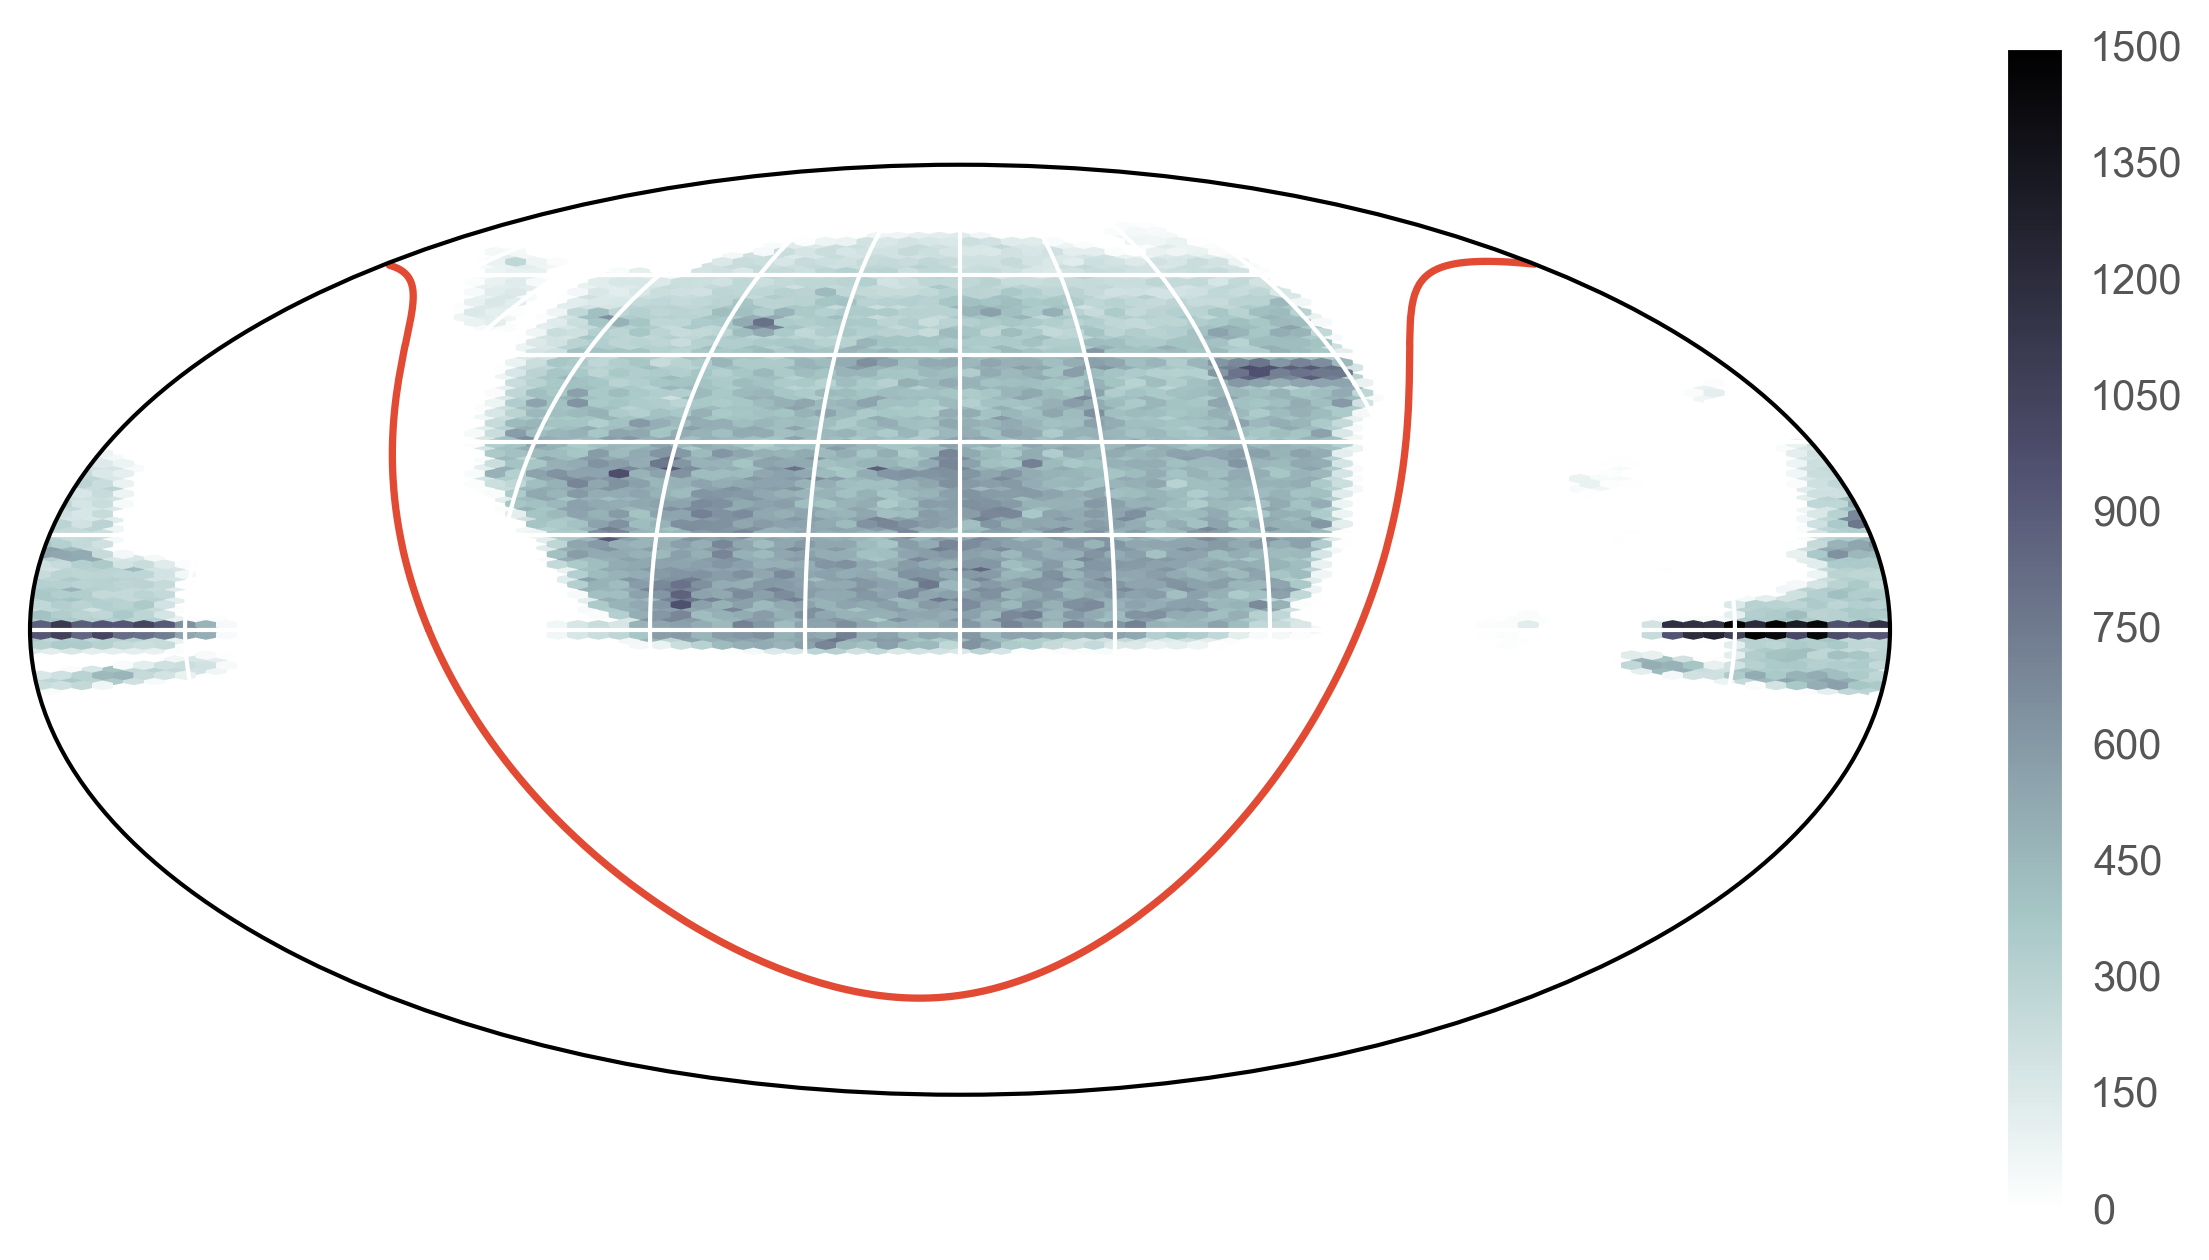
\includegraphics[width=0.73\textwidth]{figures/4_expt1/sdss_train_galaxies}
		\caption{The distribution of galaxies.}
		\label{fig:training_g}
	\end{subfigure}\\
	\begin{subfigure}{\textwidth}
		\centering
		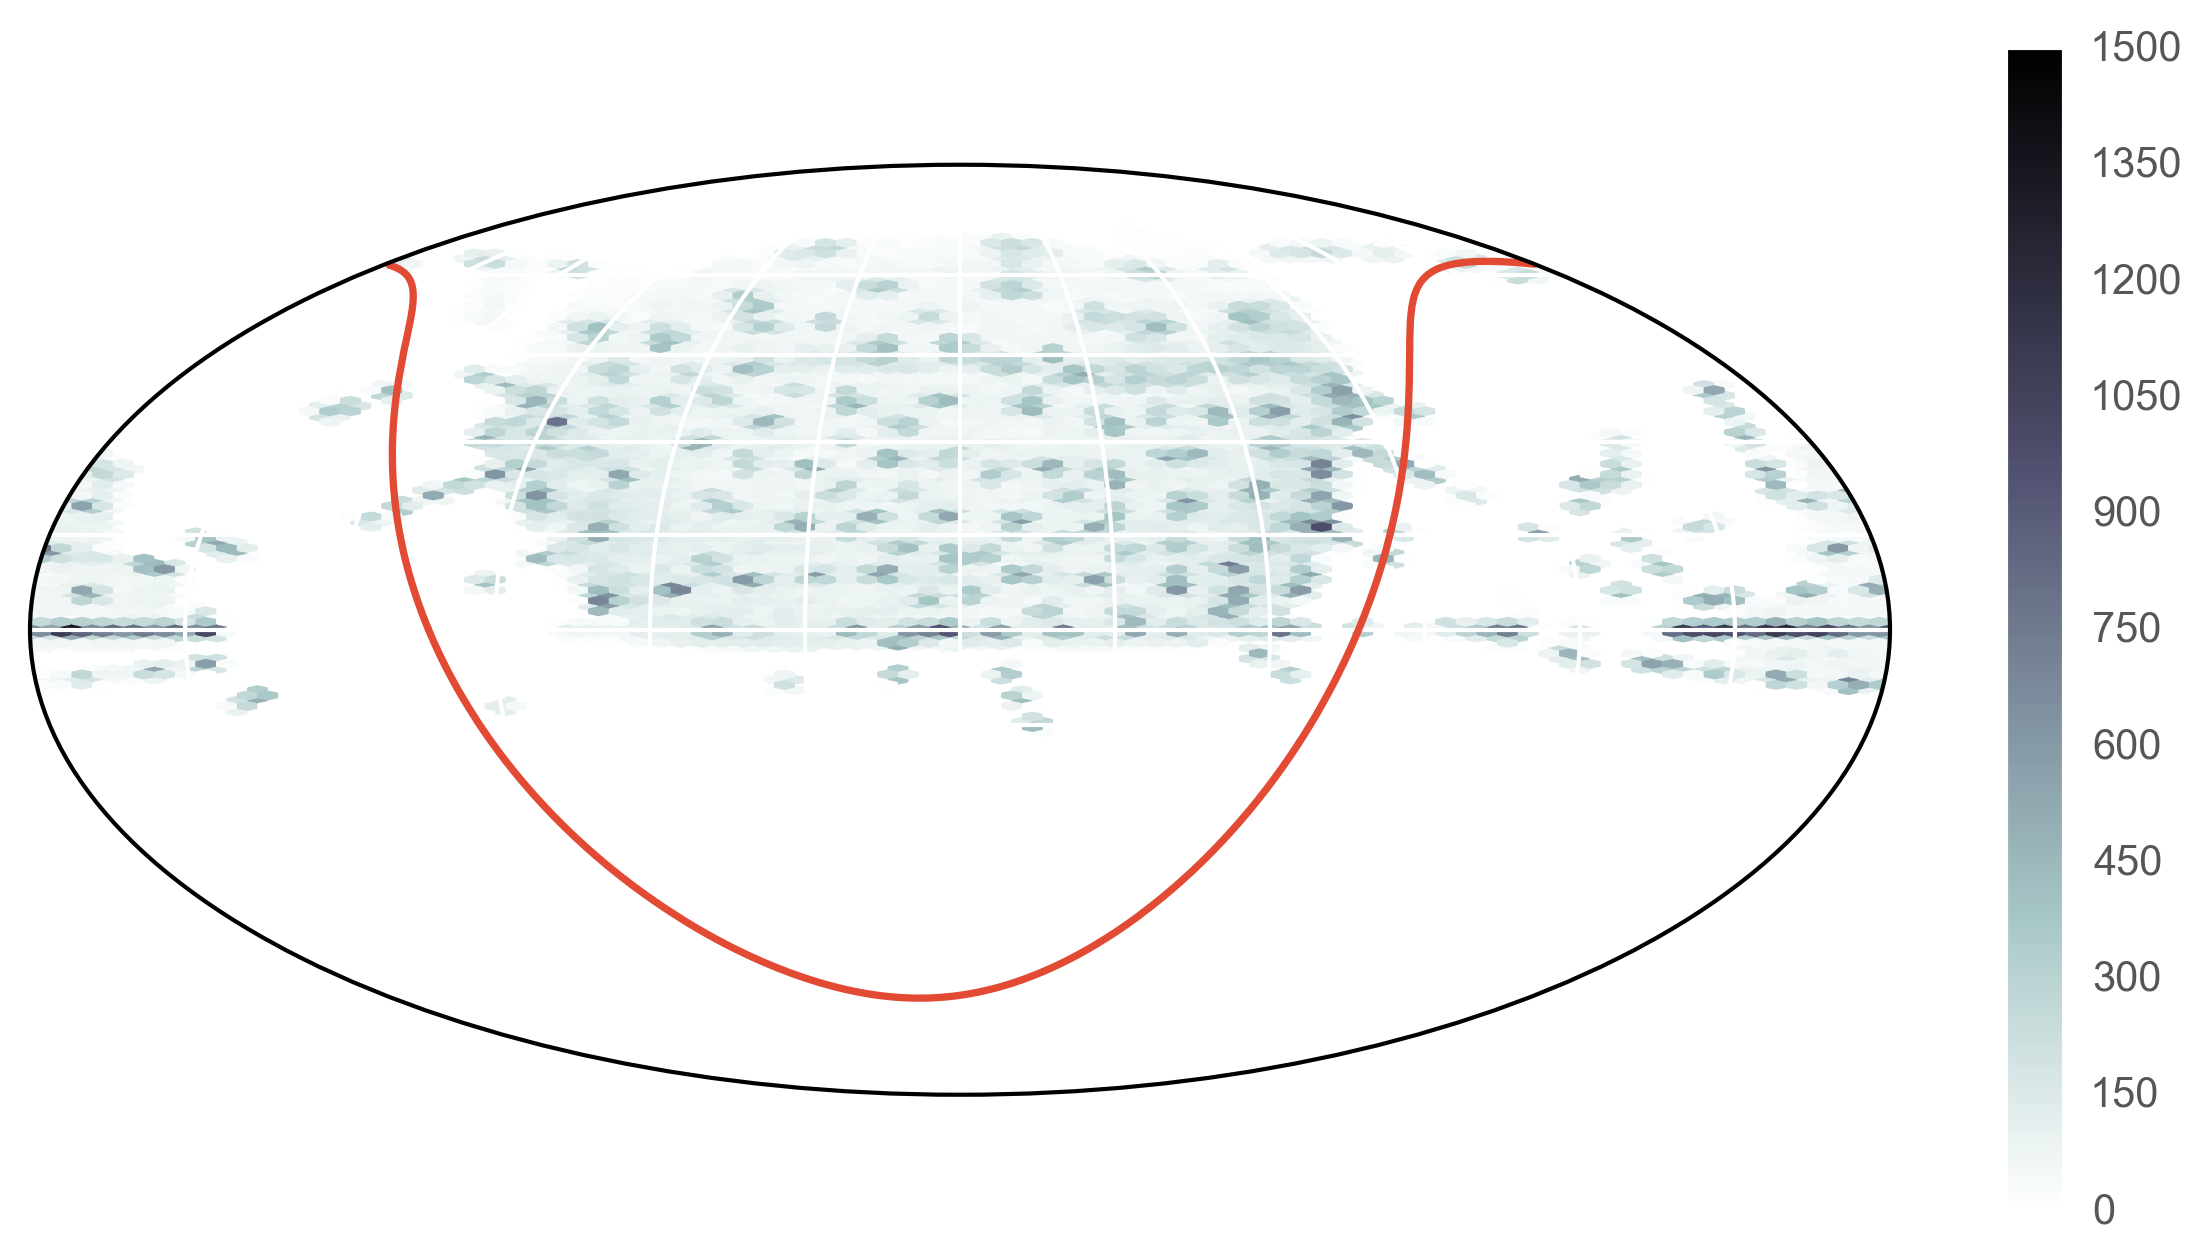
\includegraphics[width=0.73\linewidth]{figures/4_expt1/sdss_train_stars}
		\caption{The distribution of stars.}
		\label{fig:training_s}
	\end{subfigure}
	\begin{subfigure}{\textwidth}
		\centering
		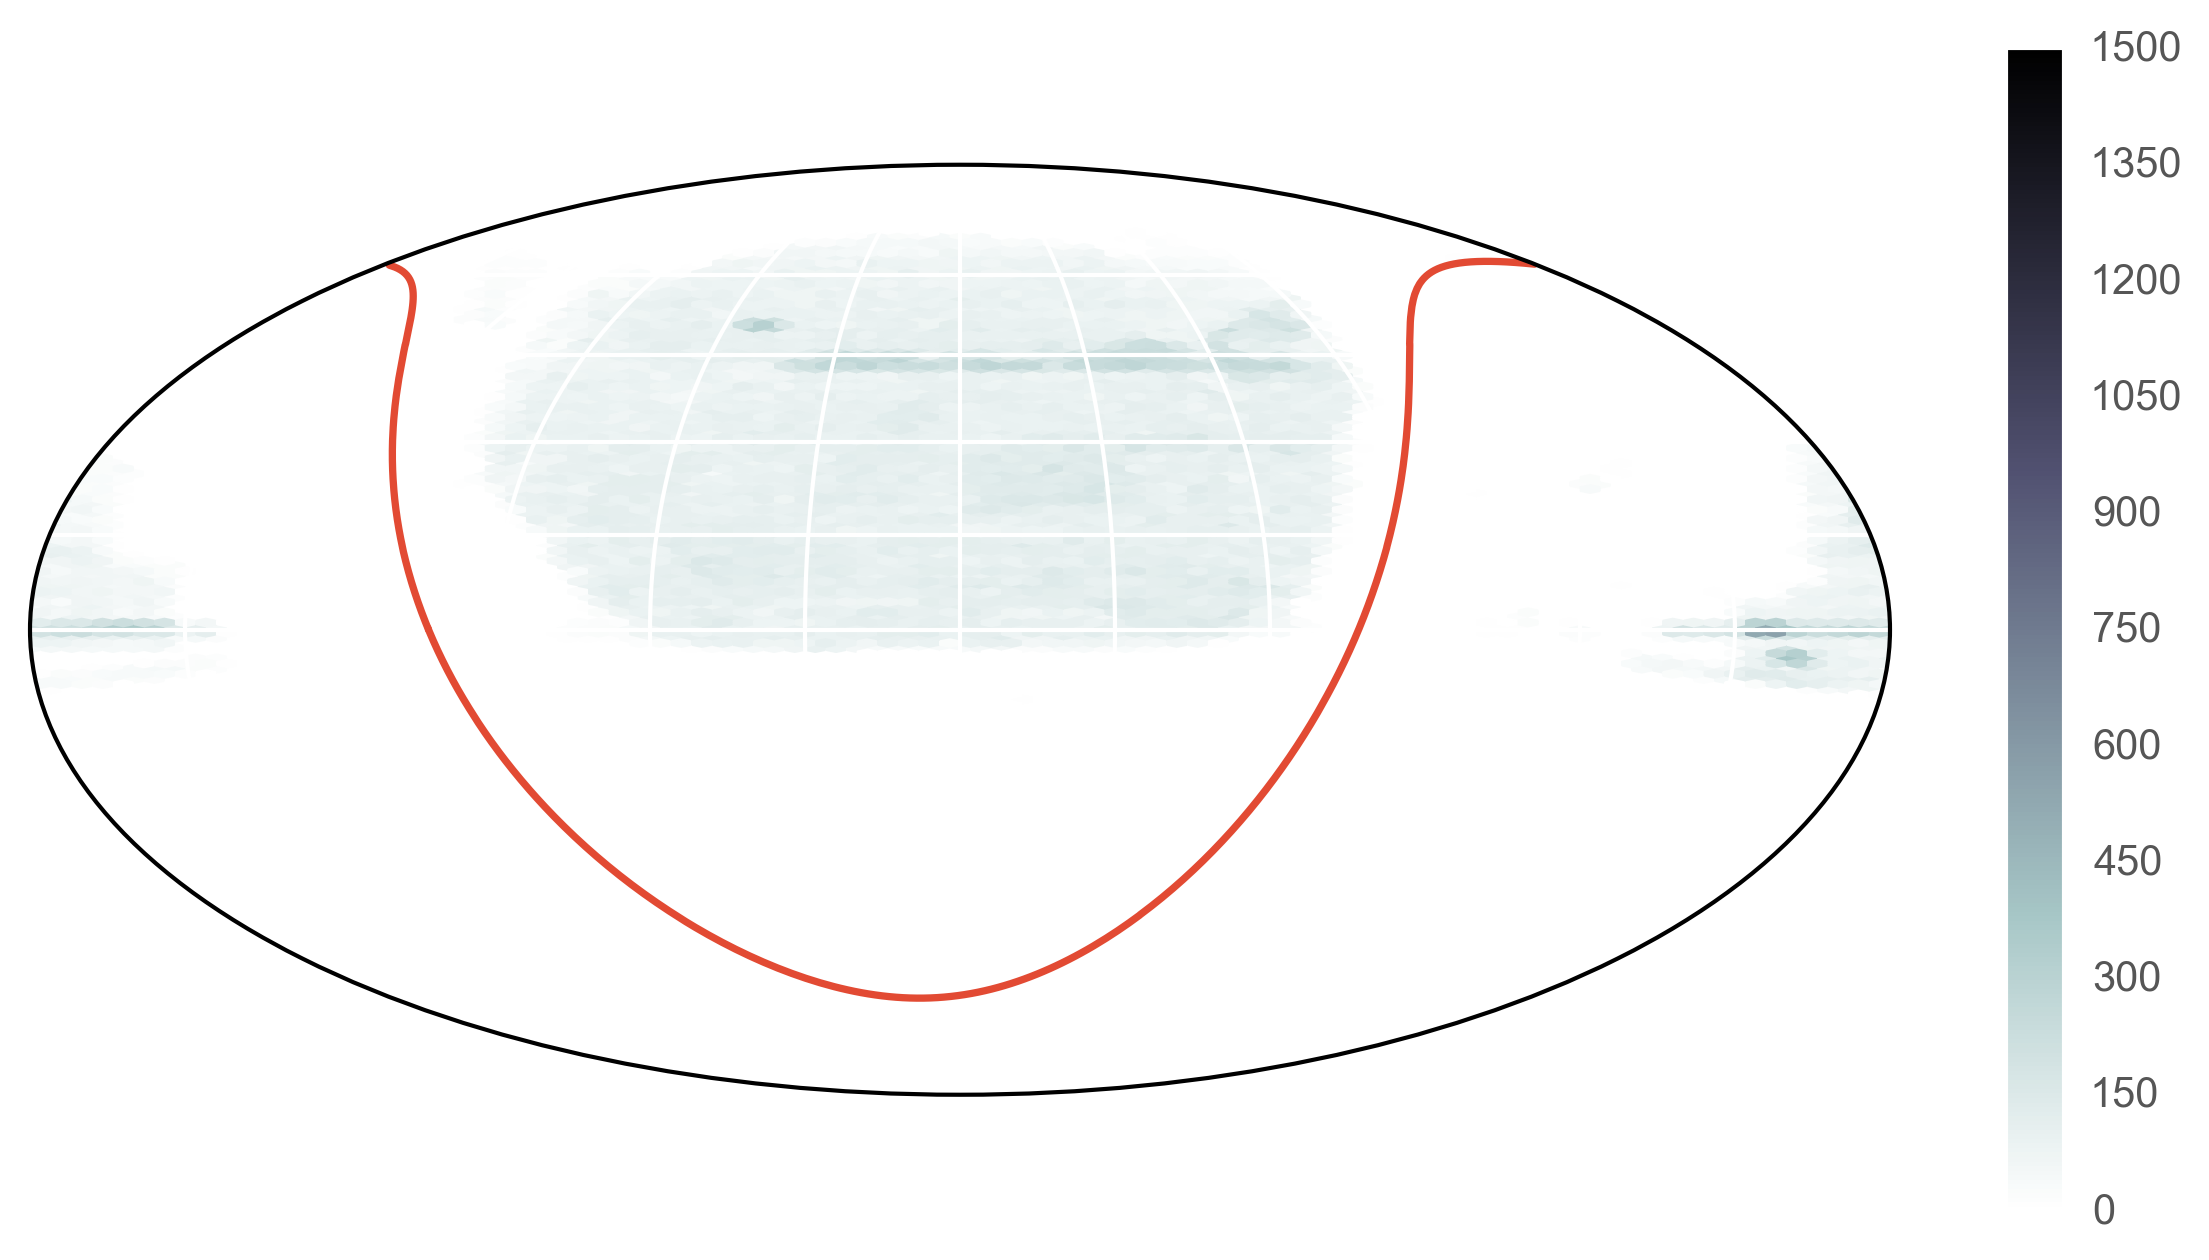
\includegraphics[width=0.73\linewidth]{figures/4_expt1/sdss_train_quasars}
		\caption{The distribution of quasars.}
		\label{fig:training_q}
	\end{subfigure}
	\caption[Distribution map of labelled objects in the SDSS]{The distribution map of
		the 2.8 million labelled objects in the SDSS: Observe that the
		galaxies are mostly uniformly distributed in the survey, while the stars are not.
		We also do not have a lot of examples of quasars.}
	\label{fig:training_dist}
\end{figure}

\begin{figure}[p]
	\centering
	\begin{subfigure}{\textwidth}
		\centering
		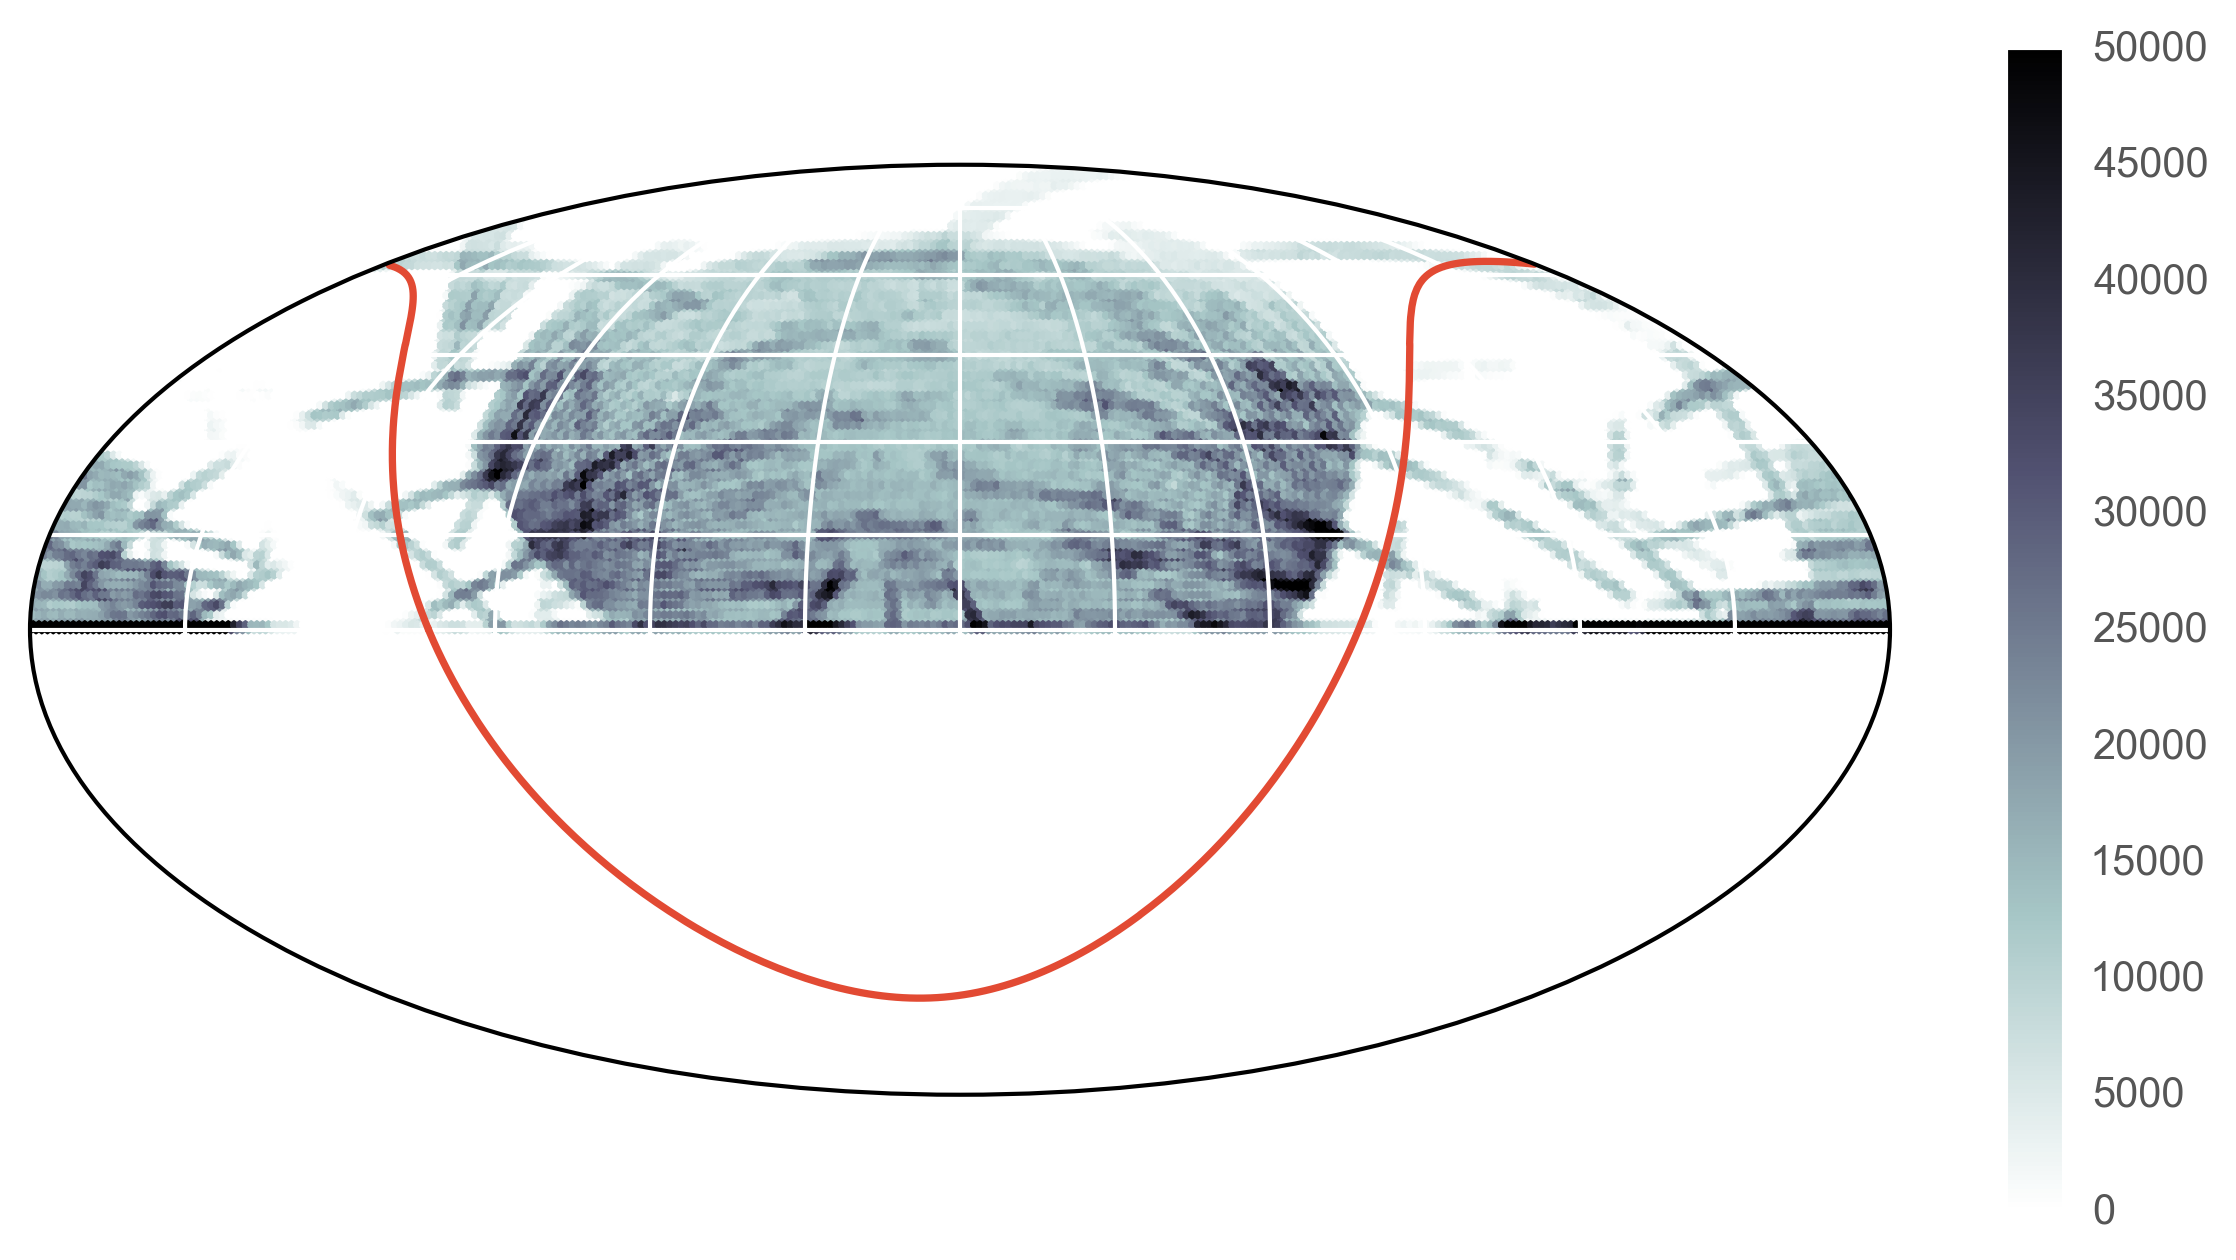
\includegraphics[width=0.75\textwidth]{figures/4_expt1/map_prediction_forest_galaxies}
		\caption{Distribution of galaxies.}
		\label{fig:random1}
	\end{subfigure}\\
	\begin{subfigure}{\textwidth}
		\centering
		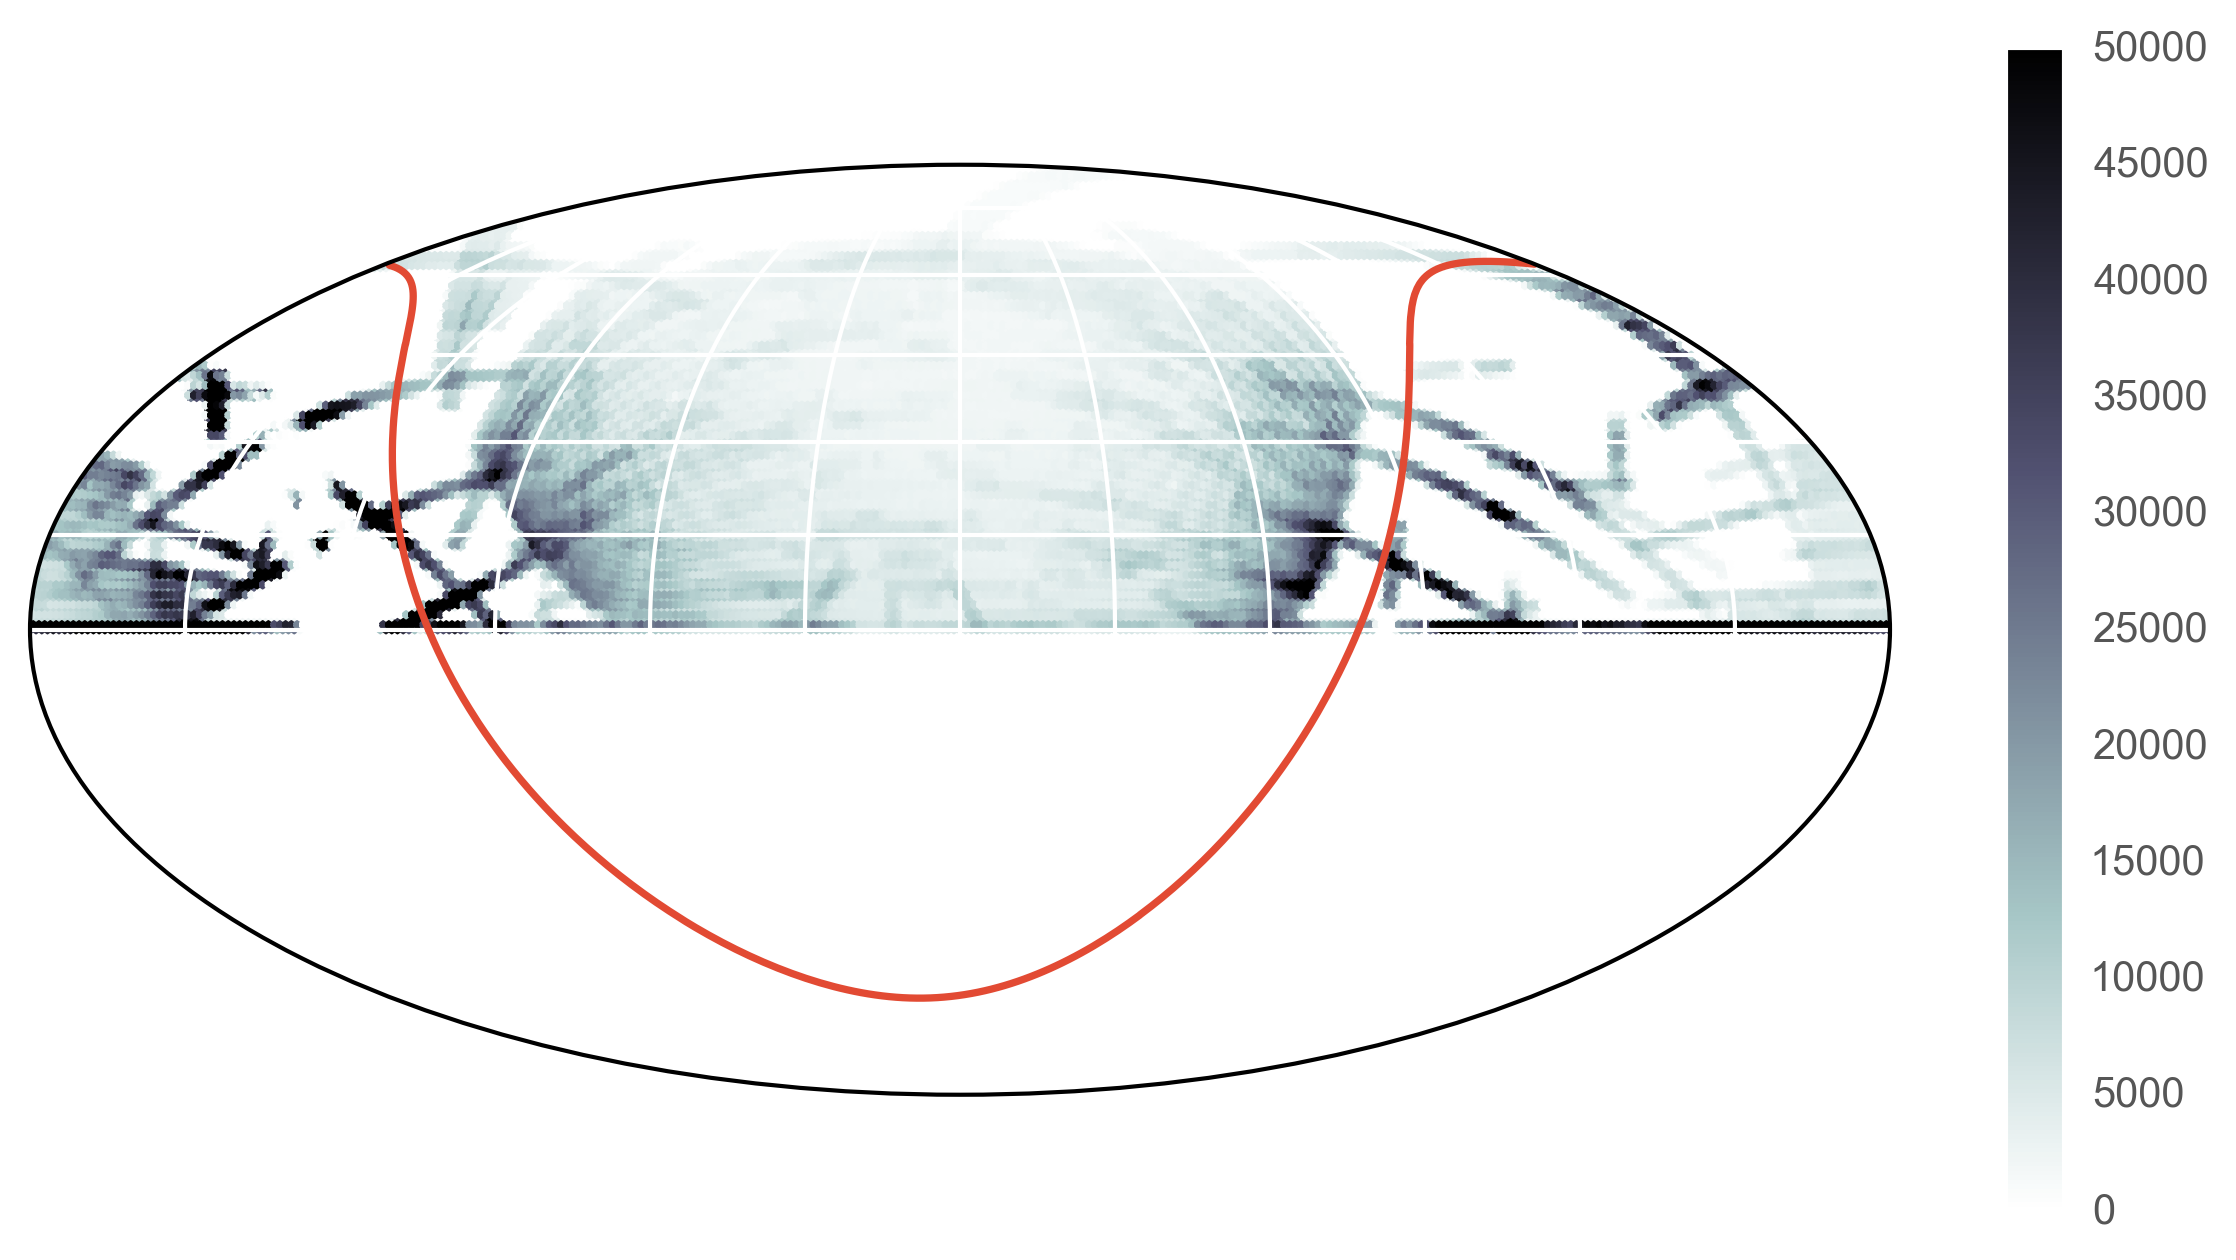
\includegraphics[width=0.75\linewidth]{figures/4_expt1/map_prediction_forest_stars}
		\caption{Distribution of stars.}
		\label{fig:random2}
	\end{subfigure}
	\begin{subfigure}{\textwidth}
		\centering
		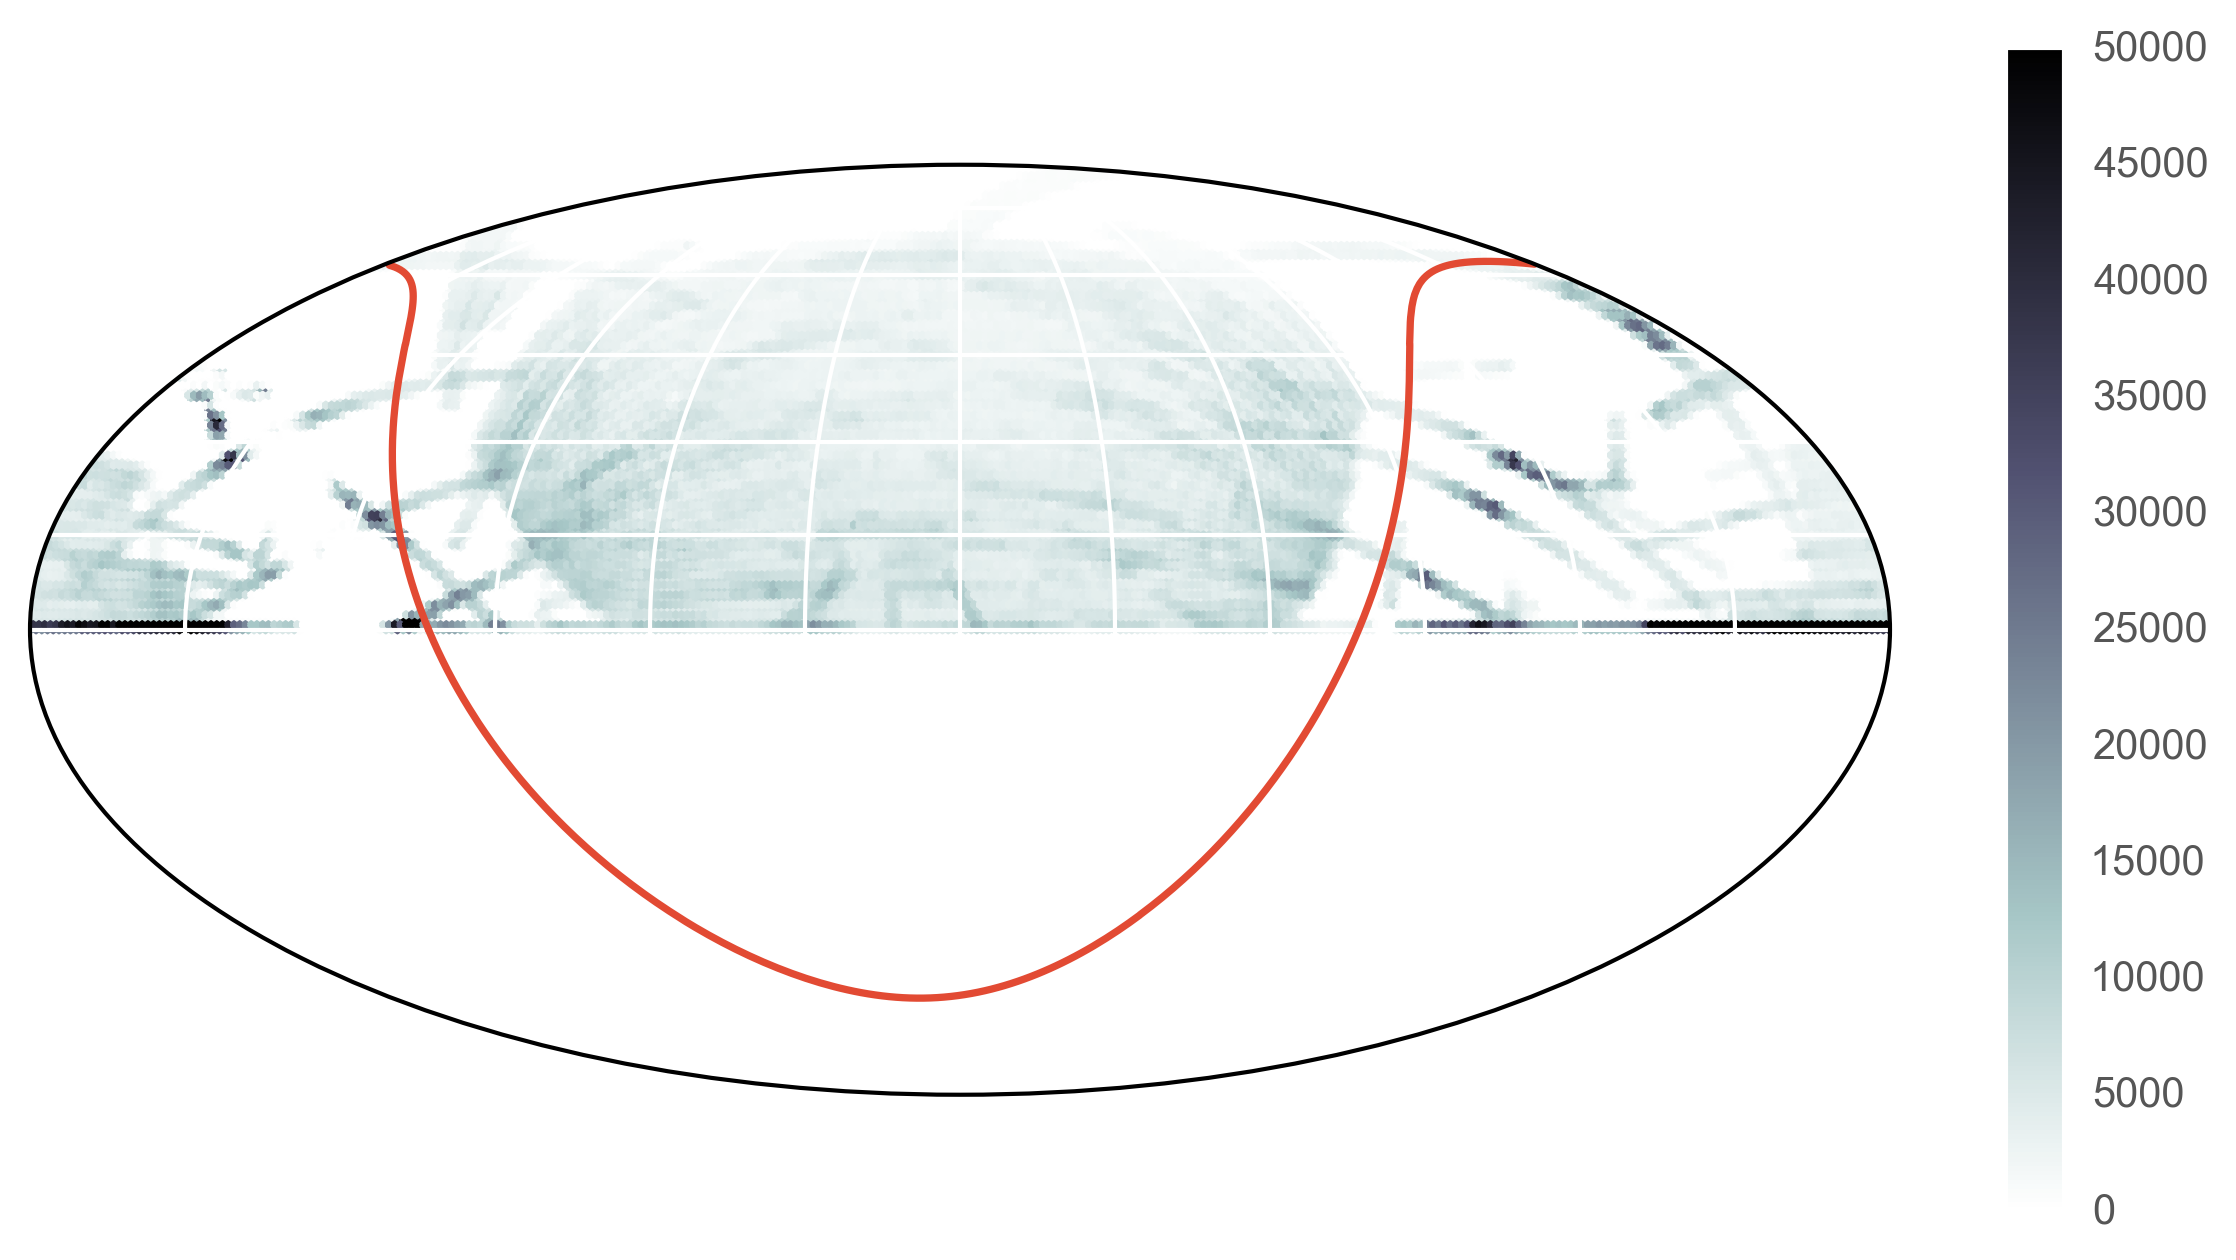
\includegraphics[width=0.75\linewidth]{figures/4_expt1/map_prediction_forest_quasars}
		\caption{Distribution of quasars.}
		\label{fig:random3}
	\end{subfigure}
	\caption[Map of predicted labels on the whole SDSS dataset using random forest.]{
		Map of predicted labels on the whole SDSS dataset using random forest.}
	\label{fig:forest}
\end{figure}


\begin{figure}[p]
	\centering
	\begin{subfigure}{\textwidth}
		\centering
		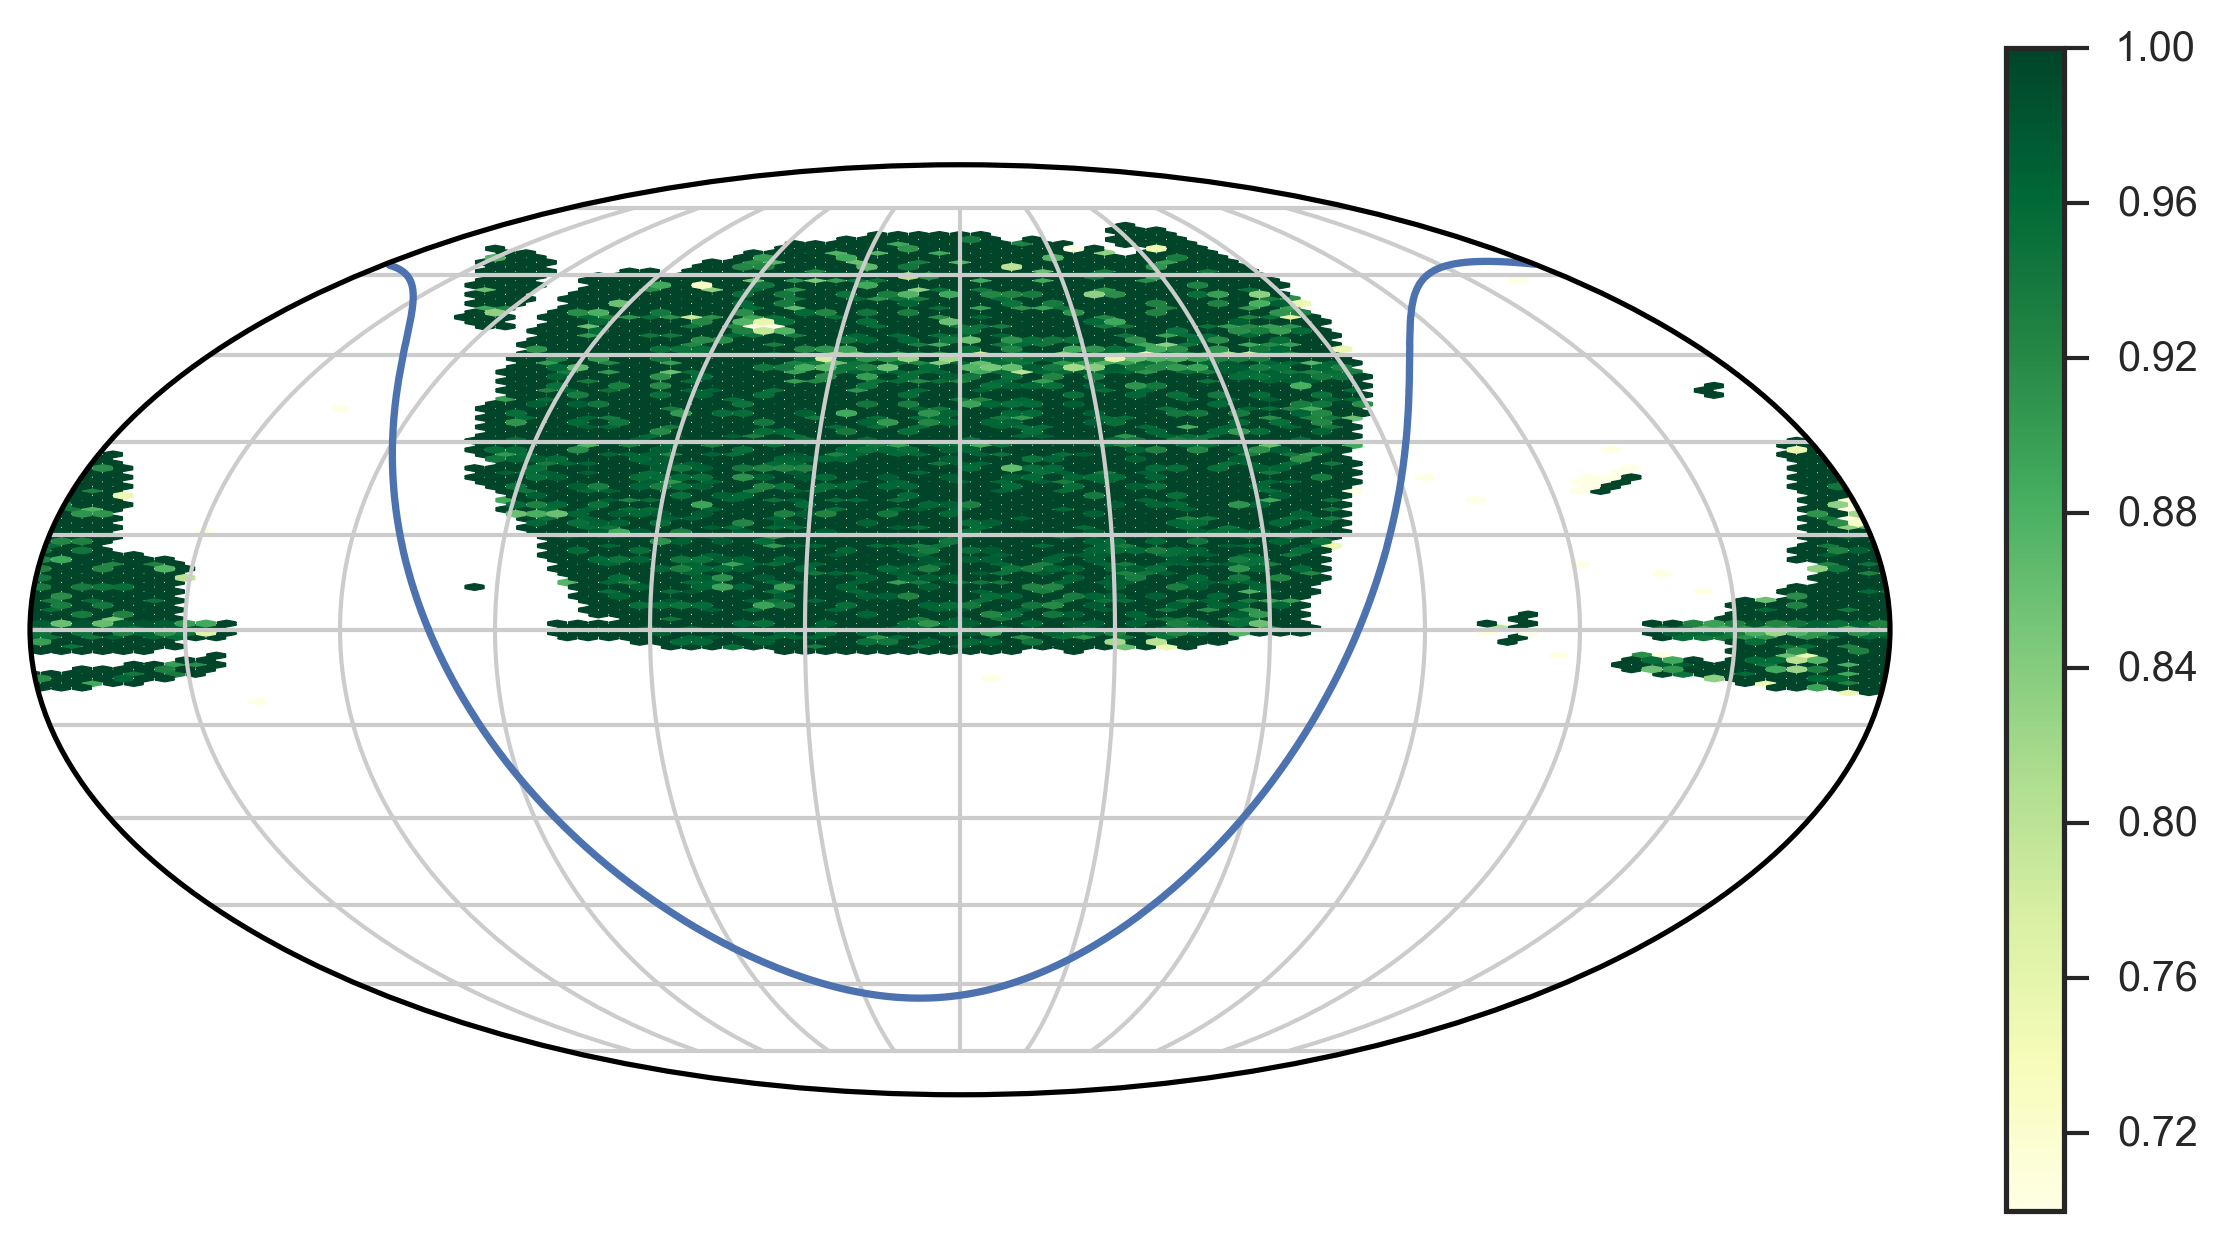
\includegraphics[width=0.75\textwidth]{figures/4_expt1/map_recall_forest_all_Galaxy}
		\caption{Recall of galaxies.}
		\label{fig:map_recall_forest_all_Galaxy}
	\end{subfigure}\\
	\begin{subfigure}{\textwidth}
		\centering
		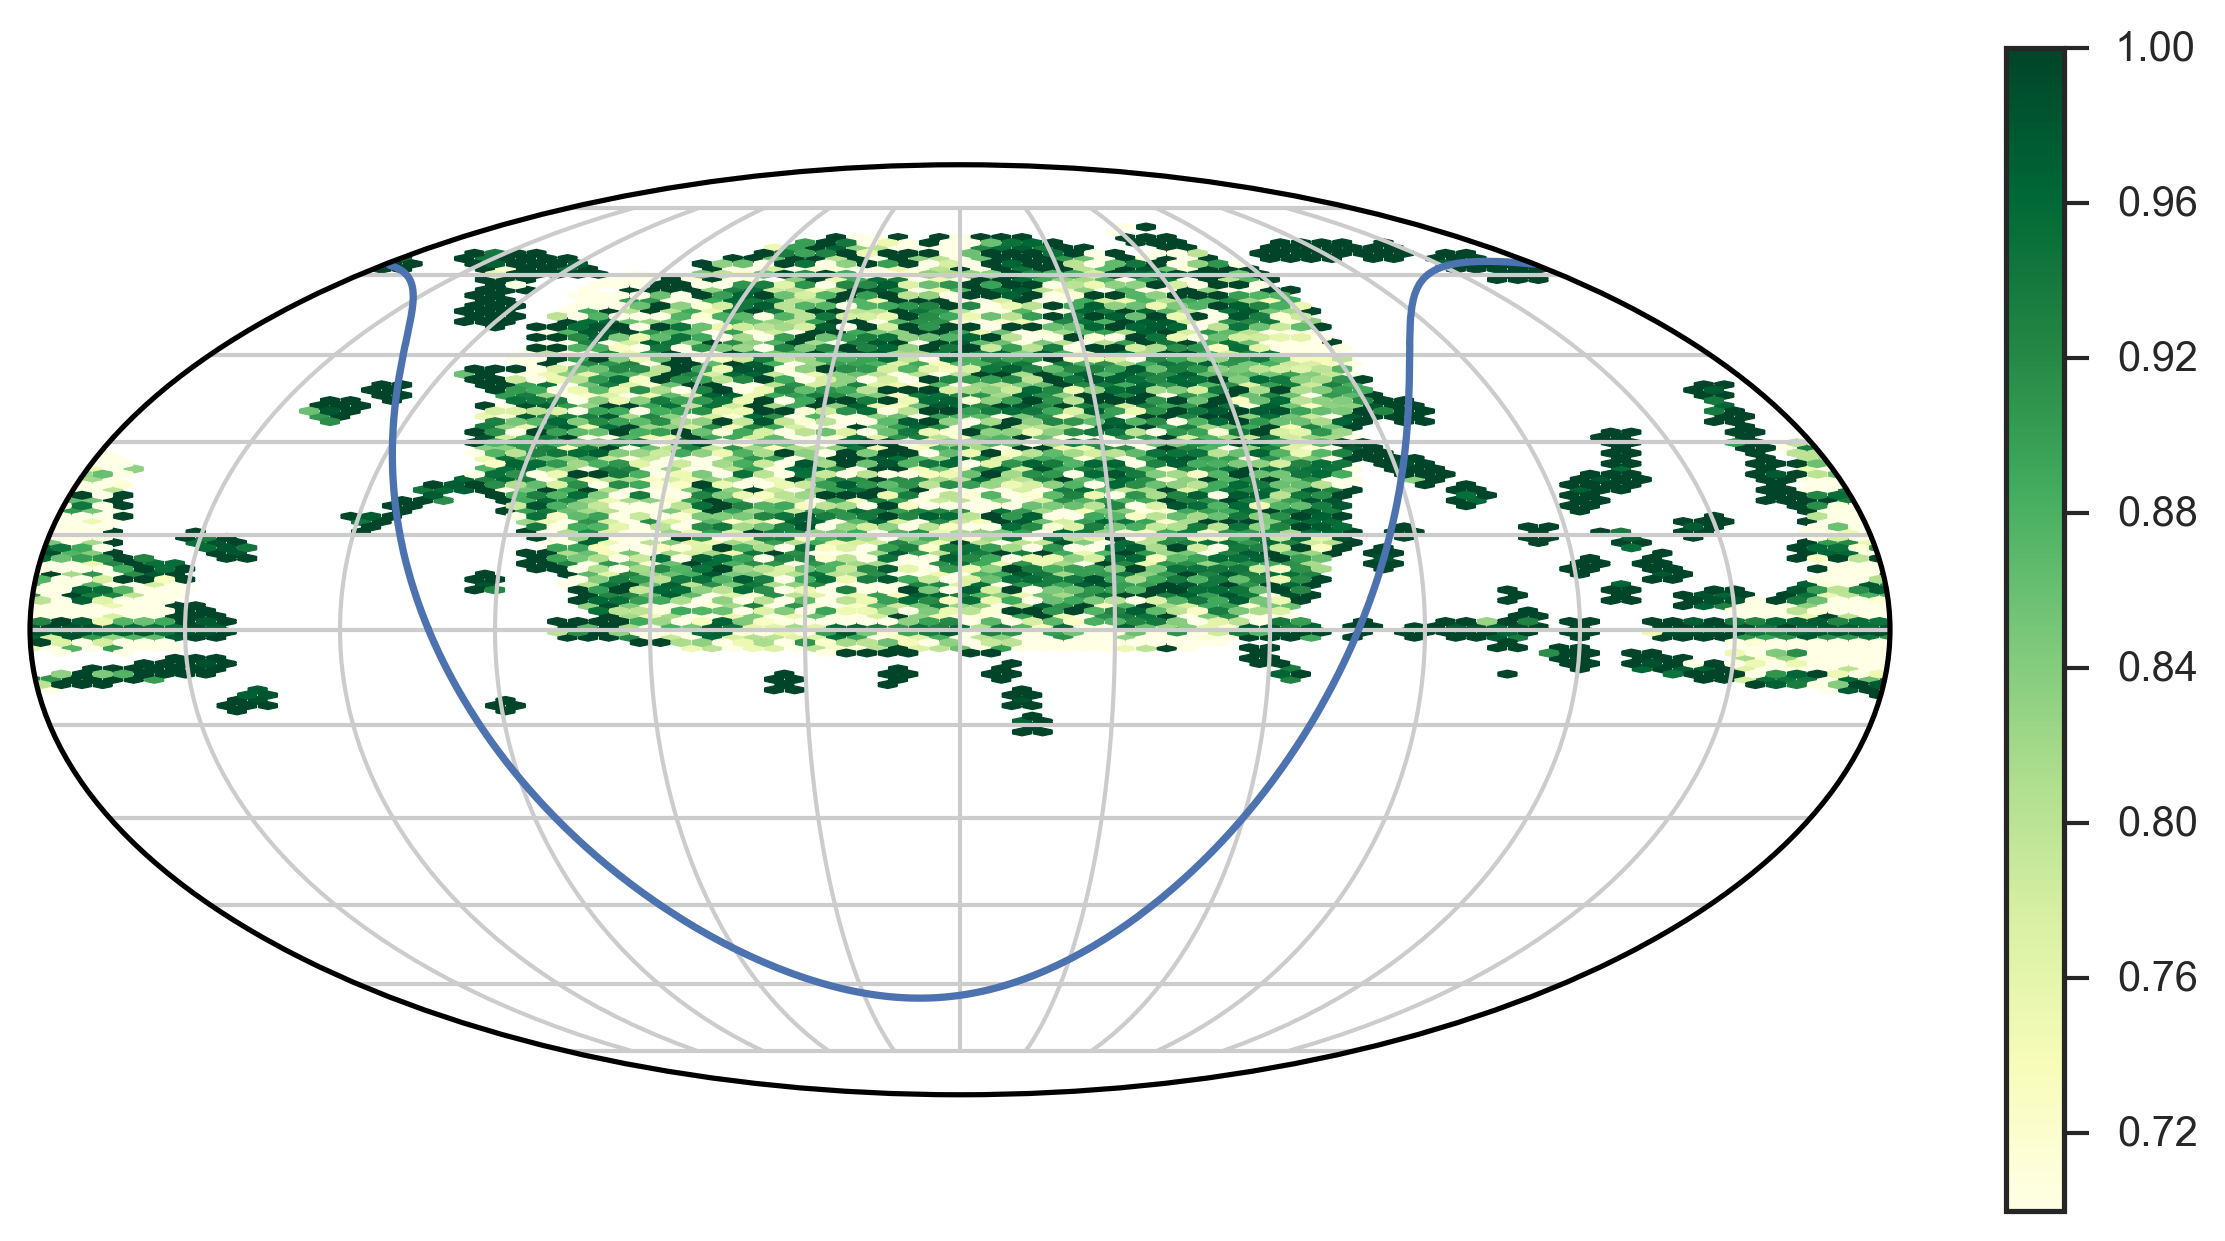
\includegraphics[width=0.75\linewidth]{figures/4_expt1/map_recall_forest_all_Star}
		\caption{Recall of stars.}
		\label{fig:map_recall_forest_all_Star}
	\end{subfigure}
	\begin{subfigure}{\textwidth}
		\centering
		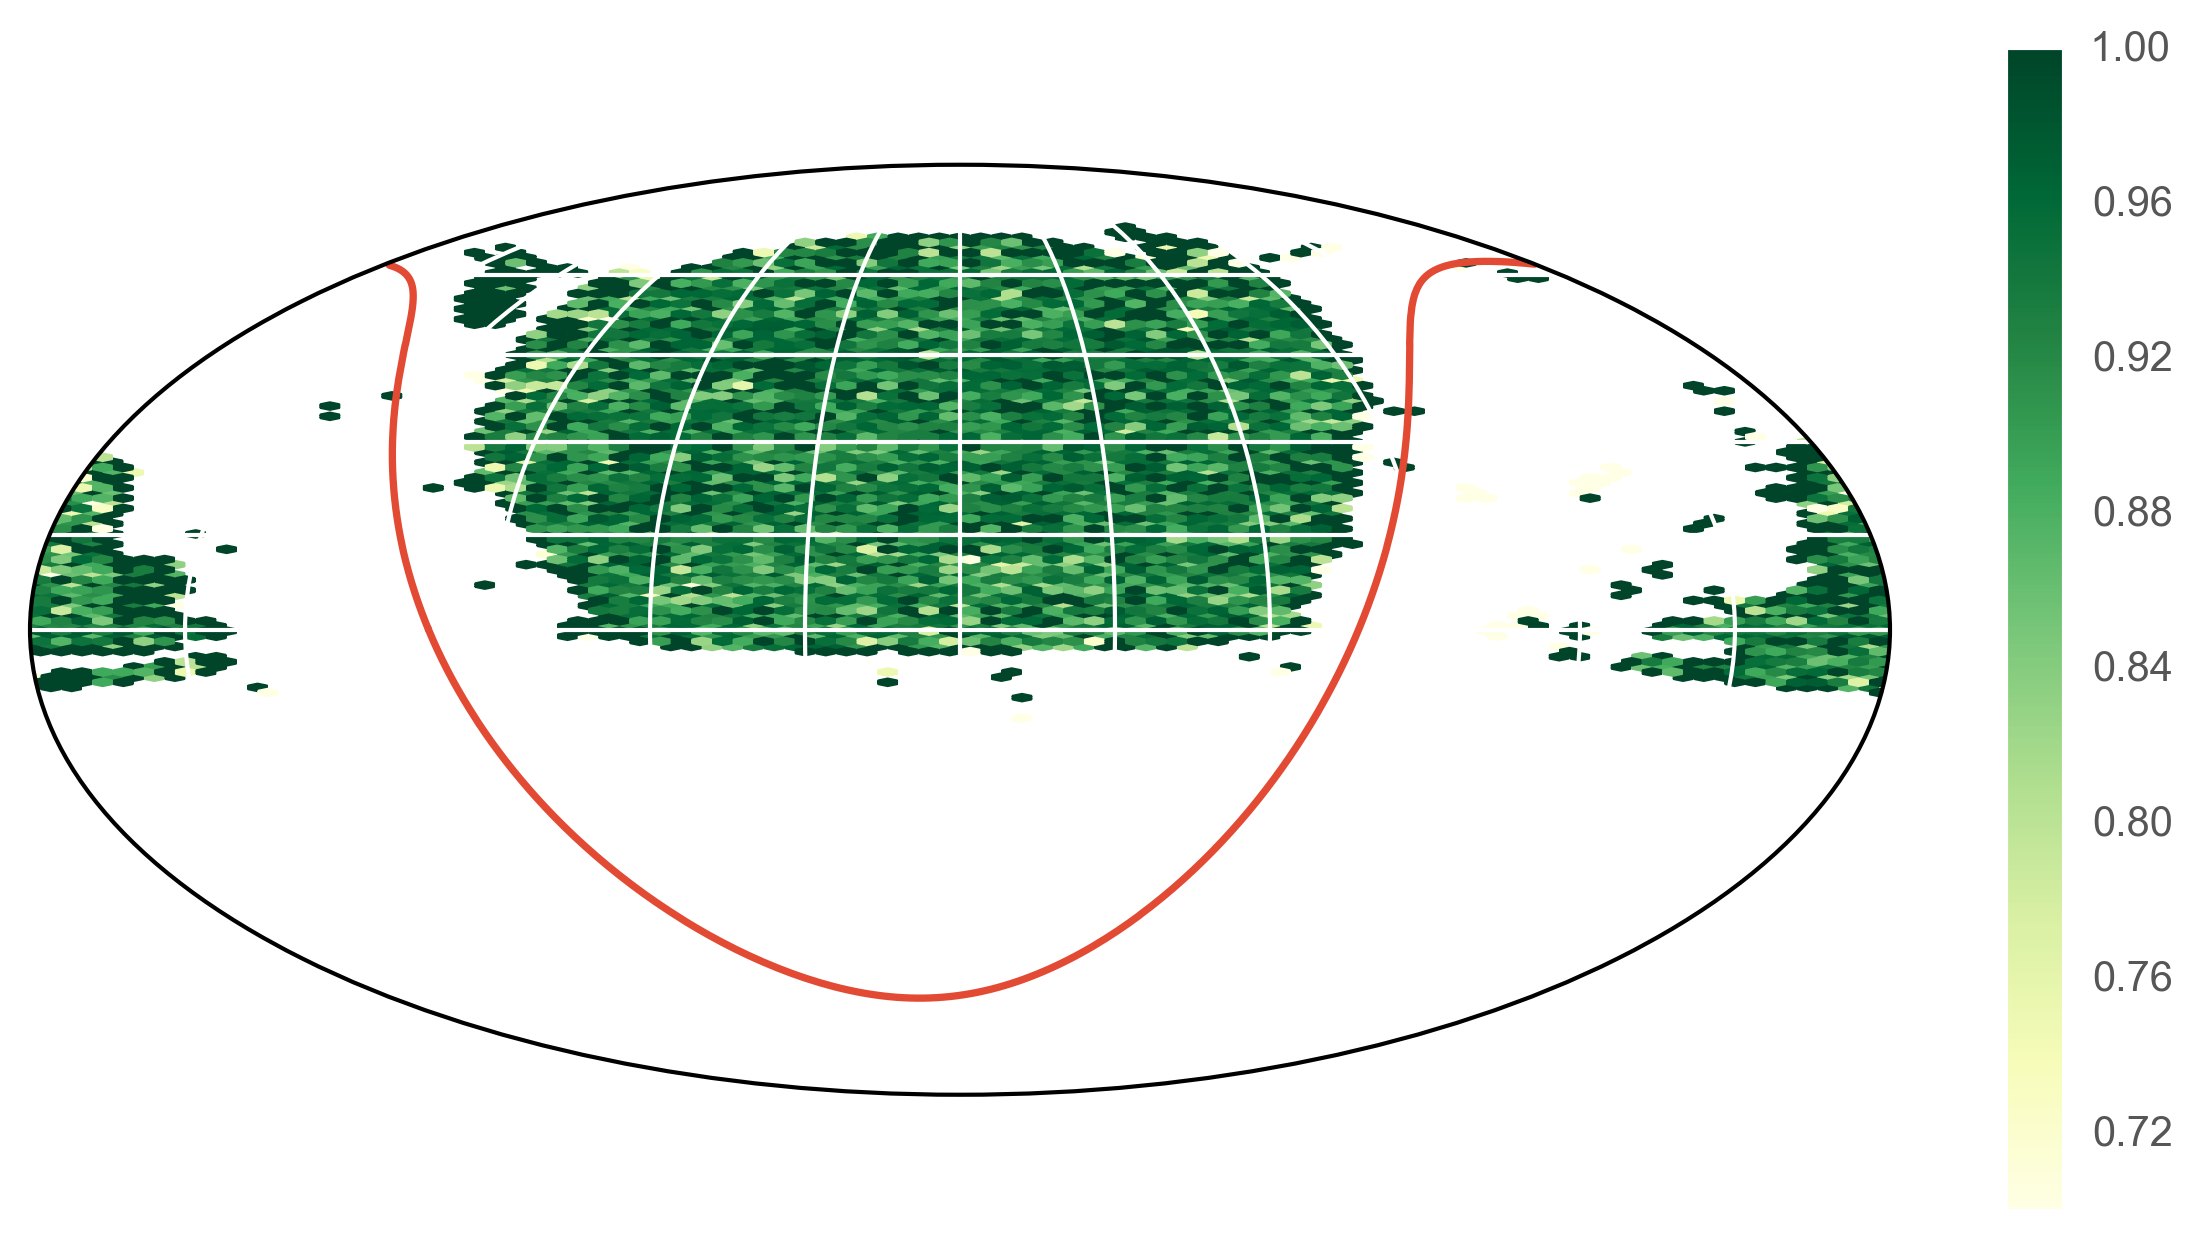
\includegraphics[width=0.75\linewidth]{figures/4_expt1/map_recall_forest_all_Quasar}
		\caption{Recall of quasars.}
		\label{fig:map_recall_forest_all_Quasar}
	\end{subfigure}
	\caption{Recall map of the random forest.}
	\label{fig:map_recall_forest_all}
\end{figure}



%%% Local Variables: 
%%% mode: latex
%%% TeX-master: "thesis"
%%% End: 
